\documentclass[]{article}
\usepackage{lmodern}
\usepackage{amssymb,amsmath}
\usepackage{ifxetex,ifluatex}
\usepackage{fixltx2e} % provides \textsubscript
\ifnum 0\ifxetex 1\fi\ifluatex 1\fi=0 % if pdftex
  \usepackage[T1]{fontenc}
  \usepackage[utf8]{inputenc}
\else % if luatex or xelatex
  \ifxetex
    \usepackage{mathspec}
  \else
    \usepackage{fontspec}
  \fi
  \defaultfontfeatures{Ligatures=TeX,Scale=MatchLowercase}
\fi
% use upquote if available, for straight quotes in verbatim environments
\IfFileExists{upquote.sty}{\usepackage{upquote}}{}
% use microtype if available
\IfFileExists{microtype.sty}{%
\usepackage{microtype}
\UseMicrotypeSet[protrusion]{basicmath} % disable protrusion for tt fonts
}{}
\usepackage[margin=1in]{geometry}
\usepackage{hyperref}
\hypersetup{unicode=true,
            pdftitle={Psy/Educ 6600: Unit 5 Homework},
            pdfauthor={Your Name},
            pdfborder={0 0 0},
            breaklinks=true}
\urlstyle{same}  % don't use monospace font for urls
\usepackage{color}
\usepackage{fancyvrb}
\newcommand{\VerbBar}{|}
\newcommand{\VERB}{\Verb[commandchars=\\\{\}]}
\DefineVerbatimEnvironment{Highlighting}{Verbatim}{commandchars=\\\{\}}
% Add ',fontsize=\small' for more characters per line
\usepackage{framed}
\definecolor{shadecolor}{RGB}{248,248,248}
\newenvironment{Shaded}{\begin{snugshade}}{\end{snugshade}}
\newcommand{\KeywordTok}[1]{\textcolor[rgb]{0.13,0.29,0.53}{\textbf{#1}}}
\newcommand{\DataTypeTok}[1]{\textcolor[rgb]{0.13,0.29,0.53}{#1}}
\newcommand{\DecValTok}[1]{\textcolor[rgb]{0.00,0.00,0.81}{#1}}
\newcommand{\BaseNTok}[1]{\textcolor[rgb]{0.00,0.00,0.81}{#1}}
\newcommand{\FloatTok}[1]{\textcolor[rgb]{0.00,0.00,0.81}{#1}}
\newcommand{\ConstantTok}[1]{\textcolor[rgb]{0.00,0.00,0.00}{#1}}
\newcommand{\CharTok}[1]{\textcolor[rgb]{0.31,0.60,0.02}{#1}}
\newcommand{\SpecialCharTok}[1]{\textcolor[rgb]{0.00,0.00,0.00}{#1}}
\newcommand{\StringTok}[1]{\textcolor[rgb]{0.31,0.60,0.02}{#1}}
\newcommand{\VerbatimStringTok}[1]{\textcolor[rgb]{0.31,0.60,0.02}{#1}}
\newcommand{\SpecialStringTok}[1]{\textcolor[rgb]{0.31,0.60,0.02}{#1}}
\newcommand{\ImportTok}[1]{#1}
\newcommand{\CommentTok}[1]{\textcolor[rgb]{0.56,0.35,0.01}{\textit{#1}}}
\newcommand{\DocumentationTok}[1]{\textcolor[rgb]{0.56,0.35,0.01}{\textbf{\textit{#1}}}}
\newcommand{\AnnotationTok}[1]{\textcolor[rgb]{0.56,0.35,0.01}{\textbf{\textit{#1}}}}
\newcommand{\CommentVarTok}[1]{\textcolor[rgb]{0.56,0.35,0.01}{\textbf{\textit{#1}}}}
\newcommand{\OtherTok}[1]{\textcolor[rgb]{0.56,0.35,0.01}{#1}}
\newcommand{\FunctionTok}[1]{\textcolor[rgb]{0.00,0.00,0.00}{#1}}
\newcommand{\VariableTok}[1]{\textcolor[rgb]{0.00,0.00,0.00}{#1}}
\newcommand{\ControlFlowTok}[1]{\textcolor[rgb]{0.13,0.29,0.53}{\textbf{#1}}}
\newcommand{\OperatorTok}[1]{\textcolor[rgb]{0.81,0.36,0.00}{\textbf{#1}}}
\newcommand{\BuiltInTok}[1]{#1}
\newcommand{\ExtensionTok}[1]{#1}
\newcommand{\PreprocessorTok}[1]{\textcolor[rgb]{0.56,0.35,0.01}{\textit{#1}}}
\newcommand{\AttributeTok}[1]{\textcolor[rgb]{0.77,0.63,0.00}{#1}}
\newcommand{\RegionMarkerTok}[1]{#1}
\newcommand{\InformationTok}[1]{\textcolor[rgb]{0.56,0.35,0.01}{\textbf{\textit{#1}}}}
\newcommand{\WarningTok}[1]{\textcolor[rgb]{0.56,0.35,0.01}{\textbf{\textit{#1}}}}
\newcommand{\AlertTok}[1]{\textcolor[rgb]{0.94,0.16,0.16}{#1}}
\newcommand{\ErrorTok}[1]{\textcolor[rgb]{0.64,0.00,0.00}{\textbf{#1}}}
\newcommand{\NormalTok}[1]{#1}
\usepackage{longtable,booktabs}
\usepackage{graphicx,grffile}
\makeatletter
\def\maxwidth{\ifdim\Gin@nat@width>\linewidth\linewidth\else\Gin@nat@width\fi}
\def\maxheight{\ifdim\Gin@nat@height>\textheight\textheight\else\Gin@nat@height\fi}
\makeatother
% Scale images if necessary, so that they will not overflow the page
% margins by default, and it is still possible to overwrite the defaults
% using explicit options in \includegraphics[width, height, ...]{}
\setkeys{Gin}{width=\maxwidth,height=\maxheight,keepaspectratio}
\usepackage[normalem]{ulem}
% avoid problems with \sout in headers with hyperref:
\pdfstringdefDisableCommands{\renewcommand{\sout}{}}
\IfFileExists{parskip.sty}{%
\usepackage{parskip}
}{% else
\setlength{\parindent}{0pt}
\setlength{\parskip}{6pt plus 2pt minus 1pt}
}
\setlength{\emergencystretch}{3em}  % prevent overfull lines
\providecommand{\tightlist}{%
  \setlength{\itemsep}{0pt}\setlength{\parskip}{0pt}}
\setcounter{secnumdepth}{0}
% Redefines (sub)paragraphs to behave more like sections
\ifx\paragraph\undefined\else
\let\oldparagraph\paragraph
\renewcommand{\paragraph}[1]{\oldparagraph{#1}\mbox{}}
\fi
\ifx\subparagraph\undefined\else
\let\oldsubparagraph\subparagraph
\renewcommand{\subparagraph}[1]{\oldsubparagraph{#1}\mbox{}}
\fi

%%% Use protect on footnotes to avoid problems with footnotes in titles
\let\rmarkdownfootnote\footnote%
\def\footnote{\protect\rmarkdownfootnote}

%%% Change title format to be more compact
\usepackage{titling}

% Create subtitle command for use in maketitle
\newcommand{\subtitle}[1]{
  \posttitle{
    \begin{center}\large#1\end{center}
    }
}

\setlength{\droptitle}{-2em}
  \title{Psy/Educ 6600: Unit 5 Homework}
  \pretitle{\vspace{\droptitle}\centering\huge}
  \posttitle{\par}
\subtitle{ANOVA - With Repeated Measures}
  \author{Your Name}
  \preauthor{\centering\large\emph}
  \postauthor{\par}
  \predate{\centering\large\emph}
  \postdate{\par}
  \date{Spring 2018}


\begin{document}
\maketitle

{
\setcounter{tocdepth}{3}
\tableofcontents
}
\section{PREPARATION}\label{preparation}

\subsection{Load Packages}\label{load-packages}

Make sure the packages are \textbf{installed} \emph{(Package tab)}

\begin{Shaded}
\begin{Highlighting}[]
\KeywordTok{library}\NormalTok{(magrittr)}
\KeywordTok{library}\NormalTok{(tidyverse)    }\CommentTok{# Loads several very helpful 'tidy' packages}
\KeywordTok{library}\NormalTok{(readxl)       }\CommentTok{# Read in Excel datasets}
\KeywordTok{library}\NormalTok{(furniture)    }\CommentTok{# Nice tables (by our own Tyson Barrett)}
\KeywordTok{library}\NormalTok{(afex)         }\CommentTok{# Analysis of Factorial Experiments}
\KeywordTok{library}\NormalTok{(emmeans)      }\CommentTok{# Estimated marginal means (Least-squares means)}
\KeywordTok{library}\NormalTok{(lsmeans)      }\CommentTok{# Least-Squares Means}
\KeywordTok{library}\NormalTok{(multcomp)     }\CommentTok{# Simultaneous Inference in General Parametric Models }
\KeywordTok{library}\NormalTok{(pander)       }\CommentTok{# Formats tables }
\end{Highlighting}
\end{Shaded}

\clearpage

\subsection{Other Datasets for Section
B's}\label{other-datasets-for-section-bs}

\begin{Shaded}
\begin{Highlighting}[]
\NormalTok{audience_wide <-}\StringTok{ }\KeywordTok{data.frame}\NormalTok{(}\DataTypeTok{id     =} \DecValTok{1}\OperatorTok{:}\DecValTok{12}\NormalTok{,}
                            \DataTypeTok{one    =} \KeywordTok{c}\NormalTok{(}\DecValTok{131}\NormalTok{, }\DecValTok{109}\NormalTok{, }\DecValTok{115}\NormalTok{, }\DecValTok{110}\NormalTok{, }\DecValTok{107}\NormalTok{, }\DecValTok{111}\NormalTok{, }
                                       \DecValTok{100}\NormalTok{, }\DecValTok{115}\NormalTok{, }\DecValTok{130}\NormalTok{, }\DecValTok{118}\NormalTok{, }\DecValTok{125}\NormalTok{, }\DecValTok{135}\NormalTok{),}
                            \DataTypeTok{twenty =} \KeywordTok{c}\NormalTok{(}\DecValTok{130}\NormalTok{, }\DecValTok{124}\NormalTok{, }\DecValTok{110}\NormalTok{, }\DecValTok{108}\NormalTok{, }\DecValTok{115}\NormalTok{, }\DecValTok{117}\NormalTok{, }
                                       \DecValTok{102}\NormalTok{, }\DecValTok{120}\NormalTok{, }\DecValTok{119}\NormalTok{, }\DecValTok{122}\NormalTok{, }\DecValTok{118}\NormalTok{, }\DecValTok{130}\NormalTok{),}
                            \DataTypeTok{large  =} \KeywordTok{c}\NormalTok{(}\DecValTok{135}\NormalTok{, }\DecValTok{126}\NormalTok{, }\DecValTok{108}\NormalTok{, }\DecValTok{122}\NormalTok{, }\DecValTok{111}\NormalTok{, }\DecValTok{121}\NormalTok{, }
                                       \DecValTok{107}\NormalTok{, }\DecValTok{132}\NormalTok{, }\DecValTok{128}\NormalTok{, }\DecValTok{130}\NormalTok{, }\DecValTok{133}\NormalTok{, }\DecValTok{135}\NormalTok{))}

\NormalTok{textbook_wide <-}\StringTok{ }\KeywordTok{data.frame}\NormalTok{(}\DataTypeTok{block =} \DecValTok{1}\OperatorTok{:}\DecValTok{9}\NormalTok{,}
                            \DataTypeTok{A =} \KeywordTok{c}\NormalTok{(}\DecValTok{17}\NormalTok{,  }\DecValTok{8}\NormalTok{,  }\DecValTok{6}\NormalTok{, }\DecValTok{12}\NormalTok{, }\DecValTok{19}\NormalTok{, }\DecValTok{14}\NormalTok{, }\DecValTok{10}\NormalTok{,  }\DecValTok{7}\NormalTok{, }\DecValTok{12}\NormalTok{),}
                            \DataTypeTok{B =} \KeywordTok{c}\NormalTok{(}\DecValTok{15}\NormalTok{,  }\DecValTok{6}\NormalTok{,  }\DecValTok{5}\NormalTok{, }\DecValTok{10}\NormalTok{, }\DecValTok{20}\NormalTok{, }\DecValTok{13}\NormalTok{,  }\DecValTok{7}\NormalTok{,  }\DecValTok{7}\NormalTok{, }\DecValTok{11}\NormalTok{),}
                            \DataTypeTok{C =} \KeywordTok{c}\NormalTok{(}\DecValTok{20}\NormalTok{, }\DecValTok{11}\NormalTok{, }\DecValTok{10}\NormalTok{, }\DecValTok{14}\NormalTok{, }\DecValTok{20}\NormalTok{, }\DecValTok{15}\NormalTok{, }\DecValTok{14}\NormalTok{, }\DecValTok{11}\NormalTok{, }\DecValTok{15}\NormalTok{),}
                            \DataTypeTok{D =} \KeywordTok{c}\NormalTok{(}\DecValTok{18}\NormalTok{,  }\DecValTok{7}\NormalTok{,  }\DecValTok{6}\NormalTok{, }\DecValTok{13}\NormalTok{, }\DecValTok{18}\NormalTok{, }\DecValTok{15}\NormalTok{, }\DecValTok{10}\NormalTok{,  }\DecValTok{6}\NormalTok{, }\DecValTok{13}\NormalTok{))}

\NormalTok{memory_wide <-}\StringTok{ }\KeywordTok{data.frame}\NormalTok{(}\DataTypeTok{id =} \DecValTok{1}\OperatorTok{:}\DecValTok{6}\NormalTok{,}
                          \DataTypeTok{digit  =} \KeywordTok{c}\NormalTok{(}\DecValTok{6}\NormalTok{, }\DecValTok{8}\NormalTok{, }\DecValTok{7}\NormalTok{, }\DecValTok{8}\NormalTok{, }\DecValTok{6}\NormalTok{, }\DecValTok{7}\NormalTok{),}
                          \DataTypeTok{letter =} \KeywordTok{c}\NormalTok{(}\DecValTok{5}\NormalTok{, }\DecValTok{7}\NormalTok{, }\DecValTok{7}\NormalTok{, }\DecValTok{5}\NormalTok{, }\DecValTok{4}\NormalTok{, }\DecValTok{6}\NormalTok{),}
                          \DataTypeTok{mixed  =} \KeywordTok{c}\NormalTok{(}\DecValTok{6}\NormalTok{, }\DecValTok{5}\NormalTok{, }\DecValTok{4}\NormalTok{, }\DecValTok{8}\NormalTok{, }\DecValTok{7}\NormalTok{, }\DecValTok{5}\NormalTok{))}

\NormalTok{tasks_wide <-}\StringTok{ }\KeywordTok{data.frame}\NormalTok{(}\DataTypeTok{clerical_background   =} \KeywordTok{c}\NormalTok{(}\DecValTok{10}\NormalTok{,  }\DecValTok{7}\NormalTok{, }\DecValTok{13}\NormalTok{, }\DecValTok{18}\NormalTok{,  }\DecValTok{6}\NormalTok{),}
                         \DataTypeTok{clerical_popular      =} \KeywordTok{c}\NormalTok{(}\DecValTok{12}\NormalTok{,  }\DecValTok{9}\NormalTok{, }\DecValTok{15}\NormalTok{, }\DecValTok{12}\NormalTok{,  }\DecValTok{8}\NormalTok{),}
                         \DataTypeTok{clerical_metal        =} \KeywordTok{c}\NormalTok{( }\DecValTok{8}\NormalTok{,  }\DecValTok{4}\NormalTok{,  }\DecValTok{9}\NormalTok{,  }\DecValTok{6}\NormalTok{,  }\DecValTok{3}\NormalTok{),}
                         \DataTypeTok{mechanical_background =} \KeywordTok{c}\NormalTok{(}\DecValTok{15}\NormalTok{, }\DecValTok{19}\NormalTok{,  }\DecValTok{8}\NormalTok{, }\DecValTok{10}\NormalTok{, }\DecValTok{16}\NormalTok{),}
                         \DataTypeTok{mechanical_popular    =} \KeywordTok{c}\NormalTok{(}\DecValTok{18}\NormalTok{, }\DecValTok{22}\NormalTok{, }\DecValTok{12}\NormalTok{, }\DecValTok{10}\NormalTok{, }\DecValTok{19}\NormalTok{),}
                         \DataTypeTok{mechanical_metal      =} \KeywordTok{c}\NormalTok{(}\DecValTok{20}\NormalTok{, }\DecValTok{23}\NormalTok{, }\DecValTok{15}\NormalTok{, }\DecValTok{14}\NormalTok{, }\DecValTok{19}\NormalTok{))}

\NormalTok{anograms_wide <-}\StringTok{ }\KeywordTok{data.frame}\NormalTok{(}\DataTypeTok{none_5    =} \KeywordTok{c}\NormalTok{( }\DecValTok{9}\NormalTok{, }\DecValTok{10}\NormalTok{, }\DecValTok{12}\NormalTok{),}
                            \DataTypeTok{none_6    =} \KeywordTok{c}\NormalTok{( }\DecValTok{6}\NormalTok{,  }\DecValTok{7}\NormalTok{,  }\DecValTok{9}\NormalTok{),}
                            \DataTypeTok{none_7    =} \KeywordTok{c}\NormalTok{( }\DecValTok{4}\NormalTok{,  }\DecValTok{4}\NormalTok{,  }\DecValTok{7}\NormalTok{),}
                            \DataTypeTok{none_8    =} \KeywordTok{c}\NormalTok{( }\DecValTok{2}\NormalTok{,  }\DecValTok{3}\NormalTok{,  }\DecValTok{5}\NormalTok{),}
                            \DataTypeTok{alone_5   =} \KeywordTok{c}\NormalTok{(}\DecValTok{19}\NormalTok{, }\DecValTok{19}\NormalTok{, }\DecValTok{22}\NormalTok{),}
                            \DataTypeTok{alone_6   =} \KeywordTok{c}\NormalTok{(}\DecValTok{16}\NormalTok{, }\DecValTok{15}\NormalTok{, }\DecValTok{20}\NormalTok{),}
                            \DataTypeTok{alone_7   =} \KeywordTok{c}\NormalTok{(}\DecValTok{15}\NormalTok{, }\DecValTok{11}\NormalTok{, }\DecValTok{17}\NormalTok{),}
                            \DataTypeTok{alone_8   =} \KeywordTok{c}\NormalTok{(}\DecValTok{12}\NormalTok{, }\DecValTok{11}\NormalTok{, }\DecValTok{14}\NormalTok{),}
                            \DataTypeTok{withEgo_5 =} \KeywordTok{c}\NormalTok{(}\DecValTok{30}\NormalTok{, }\DecValTok{31}\NormalTok{, }\DecValTok{34}\NormalTok{),}
                            \DataTypeTok{withEgo_6 =} \KeywordTok{c}\NormalTok{(}\DecValTok{25}\NormalTok{, }\DecValTok{30}\NormalTok{, }\DecValTok{32}\NormalTok{),}
                            \DataTypeTok{withEgo_7 =} \KeywordTok{c}\NormalTok{(}\DecValTok{22}\NormalTok{, }\DecValTok{27}\NormalTok{, }\DecValTok{28}\NormalTok{),}
                            \DataTypeTok{withEgo_8 =} \KeywordTok{c}\NormalTok{(}\DecValTok{21}\NormalTok{, }\DecValTok{23}\NormalTok{, }\DecValTok{24}\NormalTok{))}

\NormalTok{brain_wide <-}\StringTok{ }\KeywordTok{data.frame}\NormalTok{(}\DataTypeTok{left_digit   =} \KeywordTok{c}\NormalTok{( }\DecValTok{6}\NormalTok{,  }\DecValTok{8}\NormalTok{,  }\DecValTok{7}\NormalTok{,  }\DecValTok{8}\NormalTok{,  }\DecValTok{6}\NormalTok{,  }\DecValTok{7}\NormalTok{),}
                         \DataTypeTok{left_letter  =} \KeywordTok{c}\NormalTok{( }\DecValTok{5}\NormalTok{,  }\DecValTok{7}\NormalTok{,  }\DecValTok{7}\NormalTok{,  }\DecValTok{5}\NormalTok{,  }\DecValTok{4}\NormalTok{,  }\DecValTok{6}\NormalTok{),}
                         \DataTypeTok{left_mixed   =} \KeywordTok{c}\NormalTok{( }\DecValTok{6}\NormalTok{,  }\DecValTok{5}\NormalTok{,  }\DecValTok{4}\NormalTok{,  }\DecValTok{8}\NormalTok{,  }\DecValTok{7}\NormalTok{,  }\DecValTok{5}\NormalTok{),}
                         \DataTypeTok{right_digit  =} \KeywordTok{c}\NormalTok{( }\DecValTok{9}\NormalTok{,  }\DecValTok{8}\NormalTok{,  }\DecValTok{9}\NormalTok{,  }\DecValTok{7}\NormalTok{,  }\DecValTok{7}\NormalTok{,  }\DecValTok{9}\NormalTok{),}
                         \DataTypeTok{right_letter =} \KeywordTok{c}\NormalTok{( }\DecValTok{8}\NormalTok{,  }\DecValTok{8}\NormalTok{,  }\DecValTok{7}\NormalTok{,  }\DecValTok{8}\NormalTok{,  }\DecValTok{6}\NormalTok{,  }\DecValTok{8}\NormalTok{),}
                         \DataTypeTok{right_mixed  =} \KeywordTok{c}\NormalTok{( }\DecValTok{6}\NormalTok{,  }\DecValTok{7}\NormalTok{,  }\DecValTok{8}\NormalTok{,  }\DecValTok{8}\NormalTok{,  }\DecValTok{7}\NormalTok{,  }\DecValTok{9}\NormalTok{),}
                         \DataTypeTok{none_digit   =} \KeywordTok{c}\NormalTok{( }\DecValTok{8}\NormalTok{, }\DecValTok{10}\NormalTok{,  }\DecValTok{9}\NormalTok{,  }\DecValTok{9}\NormalTok{,  }\DecValTok{8}\NormalTok{, }\DecValTok{10}\NormalTok{),}
                         \DataTypeTok{none_letter  =} \KeywordTok{c}\NormalTok{( }\DecValTok{8}\NormalTok{,  }\DecValTok{9}\NormalTok{, }\DecValTok{10}\NormalTok{,  }\DecValTok{7}\NormalTok{,  }\DecValTok{8}\NormalTok{, }\DecValTok{10}\NormalTok{),}
                         \DataTypeTok{none_mixed   =} \KeywordTok{c}\NormalTok{( }\DecValTok{7}\NormalTok{,  }\DecValTok{9}\NormalTok{,  }\DecValTok{8}\NormalTok{,  }\DecValTok{9}\NormalTok{,  }\DecValTok{8}\NormalTok{,  }\DecValTok{9}\NormalTok{))}
\end{Highlighting}
\end{Shaded}

\clearpage

\subsection{Ihno's Dataset for Section
C's}\label{ihnos-dataset-for-section-cs}

Import Data, Define Factors, and Compute New Variables

\begin{itemize}
\tightlist
\item
  Make sure the \textbf{dataset} is saved in the same \emph{folder} as
  this file
\item
  Make sure the that \emph{folder} is the \textbf{working directory}
\end{itemize}

\begin{quote}
NOTE: I added the second line to convert all the variables names to
lower case. I still kept the \texttt{F} as a capital letter at the end
of the five factor variables.
\end{quote}

\begin{Shaded}
\begin{Highlighting}[]
\NormalTok{ihno_clean <-}\StringTok{ }\KeywordTok{read_excel}\NormalTok{(}\StringTok{"Ihno_dataset.xls"}\NormalTok{) }\OperatorTok\StringTok{ }
\StringTok{  }\NormalTok{dplyr}\OperatorTok{::}\KeywordTok{rename_all}\NormalTok{(tolower) }\OperatorTok\StringTok{ }
\StringTok{  }\NormalTok{dplyr}\OperatorTok{::}\KeywordTok{mutate}\NormalTok{(}\DataTypeTok{genderF =} \KeywordTok{factor}\NormalTok{(gender, }
                                 \DataTypeTok{levels =} \KeywordTok{c}\NormalTok{(}\DecValTok{1}\NormalTok{, }\DecValTok{2}\NormalTok{),}
                                 \DataTypeTok{labels =} \KeywordTok{c}\NormalTok{(}\StringTok{"Female"}\NormalTok{, }
                                            \StringTok{"Male"}\NormalTok{))) }\OperatorTok\StringTok{ }
\StringTok{  }\NormalTok{dplyr}\OperatorTok{::}\KeywordTok{mutate}\NormalTok{(}\DataTypeTok{majorF =} \KeywordTok{factor}\NormalTok{(major, }
                                \DataTypeTok{levels =} \KeywordTok{c}\NormalTok{(}\DecValTok{1}\NormalTok{, }\DecValTok{2}\NormalTok{, }\DecValTok{3}\NormalTok{, }\DecValTok{4}\NormalTok{,}\DecValTok{5}\NormalTok{),}
                                \DataTypeTok{labels =} \KeywordTok{c}\NormalTok{(}\StringTok{"Psychology"}\NormalTok{,}
                                           \StringTok{"Premed"}\NormalTok{,}
                                           \StringTok{"Biology"}\NormalTok{,}
                                           \StringTok{"Sociology"}\NormalTok{,}
                                           \StringTok{"Economics"}\NormalTok{))) }\OperatorTok\StringTok{ }
\StringTok{  }\NormalTok{dplyr}\OperatorTok{::}\KeywordTok{mutate}\NormalTok{(}\DataTypeTok{reasonF =} \KeywordTok{factor}\NormalTok{(reason,}
                                 \DataTypeTok{levels =} \KeywordTok{c}\NormalTok{(}\DecValTok{1}\NormalTok{, }\DecValTok{2}\NormalTok{, }\DecValTok{3}\NormalTok{),}
                                 \DataTypeTok{labels =} \KeywordTok{c}\NormalTok{(}\StringTok{"Program requirement"}\NormalTok{,}
                                            \StringTok{"Personal interest"}\NormalTok{,}
                                            \StringTok{"Advisor recommendation"}\NormalTok{))) }\OperatorTok\StringTok{ }
\StringTok{  }\NormalTok{dplyr}\OperatorTok{::}\KeywordTok{mutate}\NormalTok{(}\DataTypeTok{exp_condF =} \KeywordTok{factor}\NormalTok{(exp_cond,}
                                   \DataTypeTok{levels =} \KeywordTok{c}\NormalTok{(}\DecValTok{1}\NormalTok{, }\DecValTok{2}\NormalTok{, }\DecValTok{3}\NormalTok{, }\DecValTok{4}\NormalTok{),}
                                   \DataTypeTok{labels =} \KeywordTok{c}\NormalTok{(}\StringTok{"Easy"}\NormalTok{,}
                                              \StringTok{"Moderate"}\NormalTok{,}
                                              \StringTok{"Difficult"}\NormalTok{,}
                                              \StringTok{"Impossible"}\NormalTok{))) }\OperatorTok\StringTok{ }
\StringTok{  }\NormalTok{dplyr}\OperatorTok{::}\KeywordTok{mutate}\NormalTok{(}\DataTypeTok{coffeeF =} \KeywordTok{factor}\NormalTok{(coffee,}
                                 \DataTypeTok{levels =} \KeywordTok{c}\NormalTok{(}\DecValTok{0}\NormalTok{, }\DecValTok{1}\NormalTok{),}
                                 \DataTypeTok{labels =} \KeywordTok{c}\NormalTok{(}\StringTok{"Not a regular coffee drinker"}\NormalTok{,}
                                            \StringTok{"Regularly drinks coffee"}\NormalTok{)))  }\OperatorTok\StringTok{ }
\StringTok{  }\NormalTok{dplyr}\OperatorTok{::}\KeywordTok{mutate}\NormalTok{(}\DataTypeTok{hr_base_bps =}\NormalTok{ hr_base }\OperatorTok{/}\StringTok{ }\DecValTok{60}\NormalTok{) }
\end{Highlighting}
\end{Shaded}

\clearpage

\section{Chapter 15: Repeated Measures
ANOVA}\label{chapter-15-repeated-measures-anova}

\subsection{\texorpdfstring{Tutorial - Fitting RM ANOVA Models with
\texttt{afex::aov\_4()}}{Tutorial - Fitting RM ANOVA Models with afex::aov\_4()}}\label{tutorial---fitting-rm-anova-models-with-afexaov_4}

The \texttt{aov\_4()} function from the \texttt{afex} package fits ANOVA
models (oneway, two-way, repeated measures, and mixed design). It needs
at least two arguments:

\begin{enumerate}
\def\labelenumi{\arabic{enumi}.}
\item
  formula:
  \texttt{continuous\_var\ \textasciitilde{}\ 1\ +\ (RM\_var\textbar{}id\_var)}
  \emph{one observation per subject for each level of the
  \texttt{RMvar}, so each \texttt{id\_var} has multiple lines for each
  subject}
\item
  dataset: \texttt{data\ =\ .} \emph{we use the period to signify that
  the datset is being piped from above}
\end{enumerate}

Here is an outline of what your syntax should look like when you
\textbf{fit and save a RM ANOVA}. Of course you will replace the dataset
name and the variable names, as well as the name you are saving it as.

\begin{quote}
\textbf{NOTE:} The \texttt{aov\_4()} function works on data in LONG
format only. Each observation needs to be on its one line or row with
seperate variables for the group membership (categorical factor or
\texttt{fct}) and the continuous measurement (numberic or \texttt{dbl}).
\end{quote}

\begin{Shaded}
\begin{Highlighting}[]
\CommentTok{# RM ANOVA: fit and save}
\NormalTok{aov_name <-}\StringTok{ }\NormalTok{data_name }\OperatorTok\StringTok{ }
\StringTok{  }\NormalTok{afex}\OperatorTok{::}\KeywordTok{aov_4}\NormalTok{(continuous_var }\OperatorTok{~}\StringTok{ }\DecValTok{1} \OperatorTok{+}\StringTok{ }\NormalTok{(RM_var}\OperatorTok{|}\NormalTok{id_var),}
              \DataTypeTok{data =}\NormalTok{ .)}
\end{Highlighting}
\end{Shaded}

\begin{center}\rule{0.5\linewidth}{\linethickness}\end{center}

By running the name you saved you model under, you will get a brief set
of output, including a measure of \textbf{Effect Size}.

\begin{quote}
\textbf{NOTE:} The \texttt{ges} is the \emph{generalized eta squared}.
In a one-way ANOVA, the eta-squared effect size is the same value, ie.
generalized \(\eta_g\) and partial \(\eta_p\) are the same.
\end{quote}

\begin{Shaded}
\begin{Highlighting}[]
\CommentTok{# Display basic ANOVA results (includes effect size)}
\NormalTok{aov_name }
\end{Highlighting}
\end{Shaded}

\clearpage

To fully fill out a standard ANOVA table and compute other effect sizes,
you will need a more complete set of output, including the \textbf{Sum
of Squares} components, you will need to add \texttt{summary()} piped at
the end of the model name before running it or after the model with a
pipe.

\begin{quote}
\textbf{NOTE:} IGNORE the first line that starts with
\texttt{(Intercept)}! Also, the `mean sum of squares' are not included
in this table, nor is the \textbf{Total} line at the bottom of the
standard ANOVA table. You will need to manually compute these values and
add them on the homework page. Remember that
\texttt{Sum\ of\ Squares\ (SS)} and \texttt{degrees\ of\ freedom\ (df)}
add up, but \texttt{Mean\ Sum\ of\ Squreas\ (MS)} do not add up. Also:
\texttt{MS\ =\ SS/df} for each term.
\end{quote}

This also runs and displays the results of Mauchly Tests for Sphericity,
as well as the Greenhouse-Geisser (GG) and Huynh-Feldt (HF) Corrections
to the p-value.

\begin{quote}
\textbf{NOTE:} If the Mauchly's p-value is bigger than .05, do not use
the corrections. If Mauchly's p-value is less than .05, then apply the
epsilon (\texttt{eps} or \(\epsilon\)) to multiply the degree's of
freedom. Yes, the df will be decimal numbers.
\end{quote}

\begin{Shaded}
\begin{Highlighting}[]
\CommentTok{# Display fuller ANOVA results (sphericity tests)}
\KeywordTok{summary}\NormalTok{(aov_name)}
\end{Highlighting}
\end{Shaded}

\begin{center}\rule{0.5\linewidth}{\linethickness}\end{center}

To see all the Sumes-of-Squared residuals for ALL of the model
comoponents, you add \texttt{\$aov} at the end of the model name.

\begin{Shaded}
\begin{Highlighting}[]
\CommentTok{# Display all the sum of squares}
\NormalTok{aov_name}\OperatorTok{$}\NormalTok{aov}
\end{Highlighting}
\end{Shaded}

\begin{center}\rule{0.5\linewidth}{\linethickness}\end{center}

Repeated Measures MANOVA Tests (Pillai test statistic) is computed is
you add \texttt{\$Anova} at the end of the model name. This is a so
called `Multivariate Test'. \textbf{This is NOT what you want to do!}

\begin{Shaded}
\begin{Highlighting}[]
\CommentTok{# Display fuller ANOVA results (includes sum of squares)}
\NormalTok{aov_name}\OperatorTok{$}\NormalTok{Anova}
\end{Highlighting}
\end{Shaded}

\clearpage

If you only need to obtain the omnibus (overall) F-test without a
correction for violation of sphericity, you can add an option for
\texttt{correction\ =\ "none"}. You can also request both the
generalized and partial \(\eta^2\) effect sizes with
\texttt{es\ =\ c("ges",\ "pes")}.

\begin{Shaded}
\begin{Highlighting}[]
\CommentTok{# RM ANOVA: no correction, both effect sizes}
\NormalTok{data_name }\OperatorTok\StringTok{ }
\StringTok{  }\NormalTok{afex}\OperatorTok{::}\KeywordTok{aov_4}\NormalTok{(continuous_var }\OperatorTok{~}\StringTok{ }\DecValTok{1} \OperatorTok{+}\StringTok{ }\NormalTok{(RM_var}\OperatorTok{|}\NormalTok{id_var),}
              \DataTypeTok{data =}\NormalTok{ .,}
              \DataTypeTok{anova_table =} \KeywordTok{list}\NormalTok{(}\DataTypeTok{correction =} \StringTok{"none"}\NormalTok{,}
                                 \DataTypeTok{es =} \KeywordTok{c}\NormalTok{(}\StringTok{"ges"}\NormalTok{, }\StringTok{"pes"}\NormalTok{)))}
\end{Highlighting}
\end{Shaded}

\begin{center}\rule{0.5\linewidth}{\linethickness}\end{center}

Post Hoc tests may be ran the same way as the 1 and 2-way ANOVAs from
the last unit.

\begin{quote}
\textbf{NOTE:} Use Fisher's LSD (\texttt{adjust\ =\ "none"}) if the
omnibus F-test is significant AND there are THREE measurements per
subject or block. Tukey's HSD (\texttt{adjust\ =\ "tukey"}) may be used
even if the F-test is not significant or if there are four or more
repeated measures.
\end{quote}

\begin{Shaded}
\begin{Highlighting}[]
\CommentTok{# RM ANOVA: post hoc all pairwise tests with Fisher's LSD correction}
\NormalTok{aov_name }\OperatorTok\StringTok{ }
\StringTok{  }\NormalTok{emmeans}\OperatorTok{::}\KeywordTok{emmeans}\NormalTok{(}\OperatorTok{~}\StringTok{ }\NormalTok{RM_var) }\OperatorTok\StringTok{ }
\StringTok{  }\KeywordTok{pairs}\NormalTok{(}\DataTypeTok{adjust =} \StringTok{"none"}\NormalTok{)}
\end{Highlighting}
\end{Shaded}

\begin{Shaded}
\begin{Highlighting}[]
\CommentTok{# RM ANOVA: post hoc all pairwise tests with Tukey's HSD correction}
\NormalTok{aov_name }\OperatorTok\StringTok{ }
\StringTok{  }\NormalTok{emmeans}\OperatorTok{::}\KeywordTok{emmeans}\NormalTok{(}\OperatorTok{~}\StringTok{ }\NormalTok{RM_var) }\OperatorTok\StringTok{ }
\StringTok{  }\KeywordTok{pairs}\NormalTok{(}\DataTypeTok{adjust =} \StringTok{"tukey"}\NormalTok{)}
\end{Highlighting}
\end{Shaded}

\begin{center}\rule{0.5\linewidth}{\linethickness}\end{center}

A means plot (model based), can help you write up your results.

\begin{quote}
\textbf{NOTE:} This zooms in on just the means and will make all
differences seem significant, so make sure to interpret it in
conjunction with the ANOVA and post hoc tests.
\end{quote}

\begin{Shaded}
\begin{Highlighting}[]
\CommentTok{# RM ANOVA: means plot}
\NormalTok{aov_name }\OperatorTok\StringTok{ }
\StringTok{  }\NormalTok{emmeans}\OperatorTok{::}\KeywordTok{emmip}\NormalTok{(}\OperatorTok{~}\StringTok{ }\NormalTok{RM_var)}
\end{Highlighting}
\end{Shaded}

\clearpage

\subsection{\texorpdfstring{\texttt{audience\_wide} - Repeated Measures
Design: Effect of Audience Size on Blood
Pressure}{audience\_wide - Repeated Measures Design: Effect of Audience Size on Blood Pressure}}\label{audience_wide---repeated-measures-design-effect-of-audience-size-on-blood-pressure}

\textbf{TEXTBOOK QUESTION:} \emph{A psychophysiologist wishes to explore
the effects of public speaking on the systolic blood pressure of young
adults. Three conditions are tested. The subject must vividly imagine
delivering a speech to one person, to a small class of 20 persons, or to
a large audience consisting of hundreds of fellow students. Each subject
has his or her systolic blood pressure measured (mmHg) under all three
conditions. Two subjects are randomly assigned to each of the six
possible treatment orders. The data appear in the following table:}

\begin{verbatim}
   id one twenty large
1   1 131    130   135
2   2 109    124   126
3   3 115    110   108
4   4 110    108   122
5   5 107    115   111
6   6 111    117   121
7   7 100    102   107
8   8 115    120   132
9   9 130    119   128
10 10 118    122   130
11 11 125    118   133
12 12 135    130   135
\end{verbatim}

\begin{center}\rule{0.5\linewidth}{\linethickness}\end{center}

Restructure from wide to long format:

\begin{verbatim}
   id audience blood_pressure
1   1      one            131
2   1   twenty            130
3   1    large            135
4   2      one            109
5   2   twenty            124
6   2    large            126
7   3      one            115
8   3   twenty            110
9   3    large            108
10  4      one            110
11  4   twenty            108
12  4    large            122
13  5      one            107
14  5   twenty            115
15  5    large            111
16  6      one            111
17  6   twenty            117
18  6    large            121
19  7      one            100
20  7   twenty            102
\end{verbatim}

\clearpage

\textbf{Summary Statistics}

\begin{longtable}[]{@{}llll@{}}
\toprule
& one & twenty & large\tabularnewline
\midrule
\endhead
& n = 12 & n = 12 & n = 12\tabularnewline
blood\_pressure & & &\tabularnewline
& 117.2 (10.9) & 117.9 (8.4) & 124.0 (10.3)\tabularnewline
\bottomrule
\end{longtable}

\textbf{Profile Plots (raw data)}

\begin{center}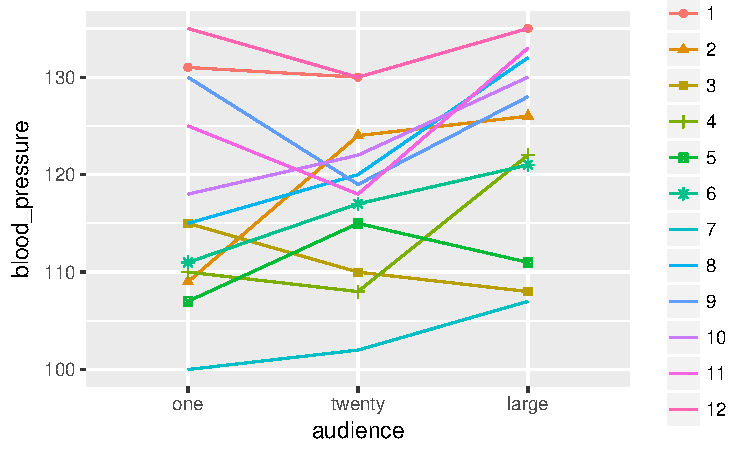
\includegraphics{Unit_5_assignment_KEY_R__spr18__files/figure-latex/unnamed-chunk-4-1} \end{center}

\textbf{Means Plot (raw data)}

\begin{center}\includegraphics{Unit_5_assignment_KEY_R__spr18__files/figure-latex/unnamed-chunk-5-1} \end{center}

\clearpage

\subsubsection{15B-3a/b/c RM ANOVA: no sphericity correction, but both
effect
sizes}\label{b-3abc-rm-anova-no-sphericity-correction-but-both-effect-sizes}

\textbf{TEXTBOOK QUESTION:} \emph{(a) Perform an RM ANOVA on the blood
pressure data and write the results in words, as they would appear in a
journal article. Does the size of the audience have a significant effect
on blood pressure at the .05 level? \sout{(Hint : Subtract 100 from
every entry in the preceding table before computing any of the SS's.
This will make your work easier without changing any of the SS
components or F ratios.)} (b) What might you do to minimize the
possibility of carryover effects?}

\textbf{DIRECTIONS:} Perform a Repeated Measures ANOVA for blood
pressure under the three condiditons to determine if the size of the
imagine audience has an effect. Request no correction for violations of
sphericity (\texttt{correction\ =\ "none"}) and both effect sizes
(\texttt{es\ =\ c("ges",\ "pes"}). Save this model as a name
\texttt{fit\_audience} and run the name (without \texttt{\$Anova}) to
see the brief output.

\begin{Shaded}
\begin{Highlighting}[]
\CommentTok{# RM ANOVA: no correction for lack of sphericity  <-- NAME AND SAVE}
\NormalTok{fit_audience <-}\StringTok{ }\NormalTok{audience_long }\OperatorTok\StringTok{ }
\StringTok{  }\NormalTok{afex}\OperatorTok{::}\KeywordTok{aov_4}\NormalTok{(blood_pressure }\OperatorTok{~}\StringTok{ }\DecValTok{1} \OperatorTok{+}\StringTok{ }\NormalTok{(audience}\OperatorTok{|}\NormalTok{id),}
              \DataTypeTok{data =}\NormalTok{ .,}
              \DataTypeTok{anova_table =} \KeywordTok{list}\NormalTok{(}\DataTypeTok{correction =} \StringTok{"none"}\NormalTok{,}
                                 \DataTypeTok{es =} \KeywordTok{c}\NormalTok{(}\StringTok{"ges"}\NormalTok{, }\StringTok{"pes"}\NormalTok{)))}

\NormalTok{fit_audience}
\end{Highlighting}
\end{Shaded}

\begin{verbatim}
Anova Table (Type 3 tests)

Response: blood_pressure
    Effect    df   MSE       F ges pes p.value
1 audience 2, 22 23.83 7.07 ** .09 .39    .004
---
Signif. codes:  0 '***' 0.001 '**' 0.01 '*' 0.05 '+' 0.1 ' ' 1
\end{verbatim}

\clearpage

\subsubsection{15B-3c RM ANOVA: display all Sums-of-Squares
components}\label{b-3c-rm-anova-display-all-sums-of-squares-components}

\textbf{TEXTBOOK QUESTION:} \emph{(c) Calculate \(\eta_{RM}^2\) from the
F ratio you calculated in part a. Does this look like a large effect?
How could this effect size be misleading in planning future
experiments?}

\textbf{DIRECTIONS:} Request all the Sums-of-Squares (SS's) by adding
\texttt{\$aov} at the end of the model name \texttt{fit\_audience}.

\begin{Shaded}
\begin{Highlighting}[]
\CommentTok{# RM ANOVA: display all Sums-of-Squares components}
\NormalTok{fit_audience}\OperatorTok{$}\NormalTok{aov}
\end{Highlighting}
\end{Shaded}

\begin{verbatim}

Call:
aov(formula = formula(paste(dv.escaped, "~", paste(c(between.escaped, 
    within.escaped), collapse = "*"), if (length(within) > 0) paste0("+Error(", 
    id.escaped, "/(", paste(within.escaped, collapse = "*"), 
    "))") else NULL)), data = dat.ret, contrasts = contrasts)

Grand Mean: 119.6944

Stratum 1: id

Terms:
                Residuals
Sum of Squares   2720.306
Deg. of Freedom        11

Residual standard error: 15.72579

Stratum 2: id:audience

Terms:
                audience Residuals
Sum of Squares  337.0556  524.2778
Deg. of Freedom        2        22

Residual standard error: 4.881681
Estimated effects may be unbalanced
\end{verbatim}

\clearpage

\subsubsection{15B-3d RM ANOVA: post hoc with Fisher's LSD
correction}\label{b-3d-rm-anova-post-hoc-with-fishers-lsd-correction}

\textbf{TEXTBOOK QUESTION:} \emph{(d) Test all the pairs of means with
protected t tests using the error term from the RM ANOVA. Which pairs
differ significantly at the .01 level?}

\textbf{DIRECTIONS:} Conduct all possible post hoc pairwise tests on
\texttt{fit\_audience} using Fisher's LSD.

\begin{Shaded}
\begin{Highlighting}[]
\CommentTok{# RM ANOVA: post hoc all pairwise tests with Fisher's LSD correction}
\NormalTok{fit_audience }\OperatorTok\StringTok{ }
\StringTok{  }\NormalTok{emmeans}\OperatorTok{::}\KeywordTok{emmeans}\NormalTok{(}\OperatorTok{~}\StringTok{ }\NormalTok{audience) }\OperatorTok\StringTok{ }
\StringTok{  }\KeywordTok{pairs}\NormalTok{(}\DataTypeTok{adjust =} \StringTok{"none"}\NormalTok{)}
\end{Highlighting}
\end{Shaded}

\begin{verbatim}
 contrast        estimate       SE df t.ratio p.value
 one - twenty   -0.750000 1.992938 22  -0.376  0.7103
 one - large    -6.833333 1.992938 22  -3.429  0.0024
 twenty - large -6.083333 1.992938 22  -3.052  0.0058
\end{verbatim}

\begin{center}\rule{0.5\linewidth}{\linethickness}\end{center}

\textbf{Means Plot (model based)}

\textbf{DIRECTIONS:} Construct a means plot of \texttt{fit\_audience}
using \texttt{emmeans::emmip(\textasciitilde{}\ RM\_var)} to help
interpret the direction of any significant differences.

\begin{Shaded}
\begin{Highlighting}[]
\CommentTok{# RM ANOVA: means plot}
\NormalTok{fit_audience }\OperatorTok\StringTok{ }
\StringTok{  }\NormalTok{emmeans}\OperatorTok{::}\KeywordTok{emmip}\NormalTok{(}\OperatorTok{~}\StringTok{ }\NormalTok{audience)}
\end{Highlighting}
\end{Shaded}

\begin{center}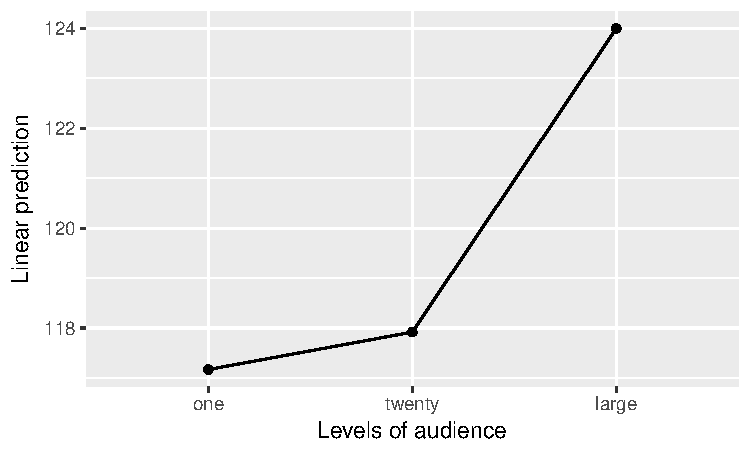
\includegraphics{Unit_5_assignment_KEY_R__spr18__files/figure-latex/unnamed-chunk-9-1} \end{center}

\clearpage

\subsection{\texorpdfstring{\texttt{textbook\_wide} - Matched Design:
Effect of Textbook on Student Quiz
Scores}{textbook\_wide - Matched Design: Effect of Textbook on Student Quiz Scores}}\label{textbook_wide---matched-design-effect-of-textbook-on-student-quiz-scores}

\textbf{TEXTBOOK QUESTION:} \emph{A statistics professor wants to know
if it really matters which textbook she uses to teach her course. She
selects four textbooks that differ in approach and then matches her 36
students into blocks of four based on their similarity in math
background and aptitude. Each student in each block is randomly assigned
to a different text. At some point in the course, the professor gives a
surprise 20-question quiz. The number of questions each student answers
correctly appears in the following table:}

\begin{verbatim}
  block  A  B  C  D
1     1 17 15 20 18
2     2  8  6 11  7
3     3  6  5 10  6
4     4 12 10 14 13
5     5 19 20 20 18
6     6 14 13 15 15
7     7 10  7 14 10
8     8  7  7 11  6
9     9 12 11 15 13
\end{verbatim}

\begin{center}\rule{0.5\linewidth}{\linethickness}\end{center}

Restructure from wide to long format:

\begin{verbatim}
   id block book quiz
1   1     1    A   17
2   2     2    A    8
3   3     3    A    6
4   4     4    A   12
5   5     5    A   19
6   6     6    A   14
7   7     7    A   10
8   8     8    A    7
9   9     9    A   12
10 10     1    B   15
11 11     2    B    6
12 12     3    B    5
13 13     4    B   10
14 14     5    B   20
15 15     6    B   13
16 16     7    B    7
17 17     8    B    7
18 18     9    B   11
19 19     1    C   20
20 20     2    C   11
\end{verbatim}

\clearpage

\textbf{Summary Statistics}

\begin{longtable}[]{@{}lllll@{}}
\toprule
& A & B & C & D\tabularnewline
\midrule
\endhead
& n = 9 & n = 9 & n = 9 & n = 9\tabularnewline
quiz & & & &\tabularnewline
& 11.7 (4.4) & 10.4 (4.9) & 14.4 (3.6) & 11.8 (4.8)\tabularnewline
\bottomrule
\end{longtable}

\textbf{Profile Plots (raw data)}

\begin{center}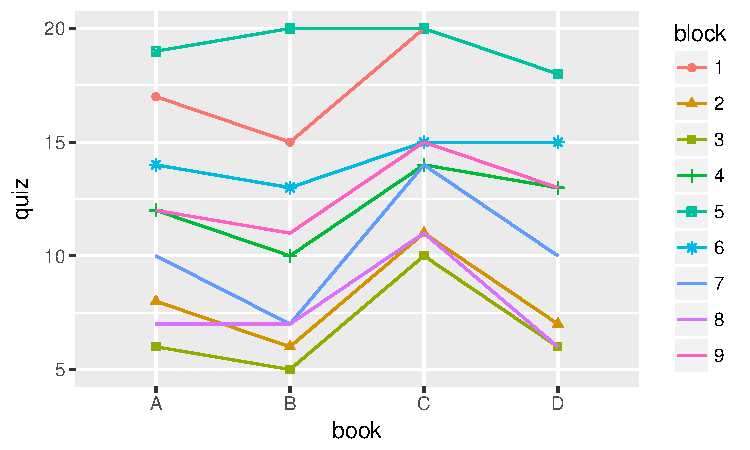
\includegraphics{Unit_5_assignment_KEY_R__spr18__files/figure-latex/unnamed-chunk-13-1} \end{center}

\textbf{Means Plots (raw data)}

\begin{center}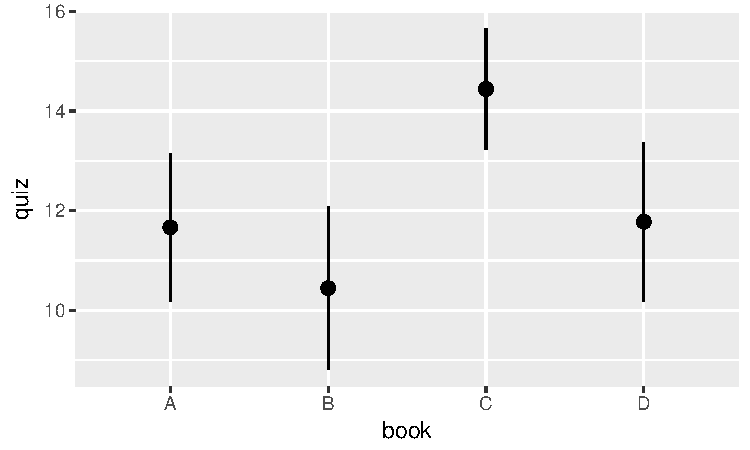
\includegraphics{Unit_5_assignment_KEY_R__spr18__files/figure-latex/unnamed-chunk-14-1} \end{center}

\clearpage

\subsubsection{15B-4a RM ANOVA: display all Sums-of-Squares
components}\label{b-4a-rm-anova-display-all-sums-of-squares-components}

\textbf{TEXTBOOK QUESTION:} \emph{(a) Perform an RM ANOVA on the data,
and present the results of your ANOVA in a summary table. Does it make a
difference which textbook the professor uses? (b) Considering your
answer to part a, what type of error could you be making (Type I or Type
II)?}

\textbf{DIRECTIONS:} Perform a Repeated Measures ANOVA for quiz scores
under the four books to determine if the text has an effect. Make sure
to save your model (\texttt{fit\_textbook}), so that you can add
\texttt{\$aov} at the end of the name to extract all the
Sums-of-Squares.

\begin{Shaded}
\begin{Highlighting}[]
\CommentTok{# RM ANOVA: display all Sums-of-Squares components}
\NormalTok{fit_textbook <-}\StringTok{ }\NormalTok{textbook_long }\OperatorTok\StringTok{ }
\StringTok{  }\NormalTok{afex}\OperatorTok{::}\KeywordTok{aov_4}\NormalTok{(quiz }\OperatorTok{~}\StringTok{ }\DecValTok{1} \OperatorTok{+}\StringTok{ }\NormalTok{(book}\OperatorTok{|}\NormalTok{block),}
              \DataTypeTok{data =}\NormalTok{ .) }

\NormalTok{fit_textbook}\OperatorTok{$}\NormalTok{aov}
\end{Highlighting}
\end{Shaded}

\begin{verbatim}

Call:
aov(formula = formula(paste(dv.escaped, "~", paste(c(between.escaped, 
    within.escaped), collapse = "*"), if (length(within) > 0) paste0("+Error(", 
    id.escaped, "/(", paste(within.escaped, collapse = "*"), 
    "))") else NULL)), data = dat.ret, contrasts = contrasts)

Grand Mean: 12.08333

Stratum 1: block

Terms:
                Residuals
Sum of Squares      612.5
Deg. of Freedom         8

Residual standard error: 8.75

Stratum 2: block:book

Terms:
                 book Residuals
Sum of Squares  76.75     27.50
Deg. of Freedom     3        24

Residual standard error: 1.070436
Estimated effects may be unbalanced
\end{verbatim}

\clearpage

\subsubsection{15B-4c RM ANOVA: GG correction for lack of
sericity}\label{b-4c-rm-anova-gg-correction-for-lack-of-sericity}

\textbf{TEXTBOOK QUESTION:} \emph{(c) Would your F ratio from part a be
significant at the .01 level if you were to assume a maximum violation
of the sphericity assumption? Explain. }

\textbf{DIRECTIONS:} Run the name of the model \texttt{fit\_textbook}
alone to extract the adjusted degrees of freedom and F-test. The
sums-of-squares for the corrected test are the same as for the
uncorrected you just did.

\begin{Shaded}
\begin{Highlighting}[]
\CommentTok{# RM ANOVA: GG correction for lack of sphericity}
\NormalTok{fit_textbook}
\end{Highlighting}
\end{Shaded}

\begin{verbatim}
Anova Table (Type 3 tests)

Response: quiz
  Effect          df  MSE         F ges p.value
1   book 2.02, 16.16 1.70 22.33 *** .11  <.0001
---
Signif. codes:  0 '***' 0.001 '**' 0.01 '*' 0.05 '+' 0.1 ' ' 1

Sphericity correction method: GG 
\end{verbatim}

\clearpage

\subsubsection{15B-4d RM ANOVA: post-hoc with Tukey's HSD
correction}\label{b-4d-rm-anova-post-hoc-with-tukeys-hsd-correction}

\textbf{TEXTBOOK QUESTION:} \emph{(d) Test all the pairs of means with
Tukey's HSD, using the error term from the RM ANOVA. Which pairs differ
significantly at the .05 level?}

\textbf{DIRECTIONS:} Conduct all possible post hoc pairwise tests on
\texttt{fit\_audience} using Tukey's HSD.

\begin{Shaded}
\begin{Highlighting}[]
\CommentTok{# RM ANOVA: post hoc all pairwise tests with Tukey's HSD correction}
\NormalTok{fit_textbook }\OperatorTok\StringTok{ }
\StringTok{  }\NormalTok{emmeans}\OperatorTok{::}\KeywordTok{emmeans}\NormalTok{(}\OperatorTok{~}\StringTok{ }\NormalTok{book) }\OperatorTok\StringTok{ }
\StringTok{  }\KeywordTok{pairs}\NormalTok{(}\DataTypeTok{adjust =} \StringTok{"tukey"}\NormalTok{)}
\end{Highlighting}
\end{Shaded}

\begin{verbatim}
 contrast   estimate        SE df t.ratio p.value
 A - B     1.2222222 0.5046084 24   2.422  0.0997
 A - C    -2.7777778 0.5046084 24  -5.505  0.0001
 A - D    -0.1111111 0.5046084 24  -0.220  0.9961
 B - C    -4.0000000 0.5046084 24  -7.927  <.0001
 B - D    -1.3333333 0.5046084 24  -2.642  0.0639
 C - D     2.6666667 0.5046084 24   5.285  0.0001

P value adjustment: tukey method for comparing a family of 4 estimates 
\end{verbatim}

\begin{center}\rule{0.5\linewidth}{\linethickness}\end{center}

\textbf{Means Plot (model based)}

\textbf{DIRECTIONS:} Construct a means plot of \texttt{fit\_audience}
using \texttt{emmeans::emmip(\textasciitilde{}\ RM\_var)} to help
interpret the direction of any significant differences.

\begin{Shaded}
\begin{Highlighting}[]
\NormalTok{textbook_long }\OperatorTok\StringTok{ }
\StringTok{  }\NormalTok{afex}\OperatorTok{::}\KeywordTok{aov_4}\NormalTok{(quiz }\OperatorTok{~}\StringTok{ }\DecValTok{1} \OperatorTok{+}\StringTok{ }\NormalTok{(book}\OperatorTok{|}\NormalTok{block),}
              \DataTypeTok{data =}\NormalTok{ .) }\OperatorTok\StringTok{ }
\StringTok{  }\NormalTok{emmeans}\OperatorTok{::}\KeywordTok{emmip}\NormalTok{(}\OperatorTok{~}\StringTok{ }\NormalTok{book)}
\end{Highlighting}
\end{Shaded}

\begin{center}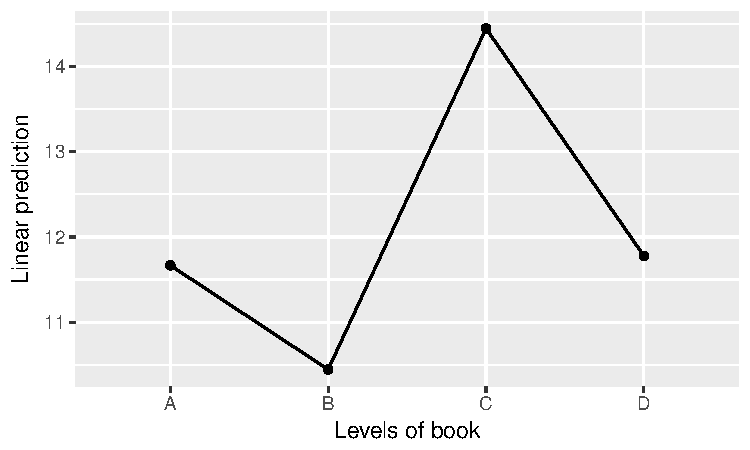
\includegraphics{Unit_5_assignment_KEY_R__spr18__files/figure-latex/unnamed-chunk-18-1} \end{center}

\clearpage

\subsubsection{15B-5a 1-Way ANOVA (treat studnets as
independent)}\label{b-5a-1-way-anova-treat-studnets-as-independent}

\textbf{TEXTBOOK QUESTION:} \emph{(a) Perform a one-way
independent-groups ANOVA on the data from Exercise 4.}

\textbf{DIRECTIONS:} Perform the ANOVA with the \texttt{book} as an
between-subjects factor, instead of a within-subjects factor (ignoring
matching) for quiz scores to determine if the text has an effect. Make
sure to save your model (\texttt{fit\_book1way}), so that you can add
\texttt{\$aov} at the end of the name to extract all the
Sums-of-Squares.

\begin{Shaded}
\begin{Highlighting}[]
\CommentTok{# 1-way ANOVA: 1 between-subject factor}
\NormalTok{fit_book1way <-}\StringTok{ }\NormalTok{textbook_long }\OperatorTok\StringTok{ }
\StringTok{  }\NormalTok{afex}\OperatorTok{::}\KeywordTok{aov_4}\NormalTok{(quiz }\OperatorTok{~}\StringTok{ }\NormalTok{book }\OperatorTok{+}\StringTok{ }\NormalTok{(}\DecValTok{1}\OperatorTok{|}\NormalTok{id),}
              \DataTypeTok{data =}\NormalTok{ .) }

\NormalTok{fit_book1way}\OperatorTok{$}\NormalTok{aov}
\end{Highlighting}
\end{Shaded}

\begin{verbatim}
Call:
   aov(formula = formula(paste(dv.escaped, "~", paste(c(between.escaped, 
    within.escaped), collapse = "*"), if (length(within) > 0) paste0("+Error(", 
    id.escaped, "/(", paste(within.escaped, collapse = "*"), 
    "))") else NULL)), data = dat.ret, contrasts = contrasts)

Terms:
                  book Residuals
Sum of Squares   76.75    640.00
Deg. of Freedom      3        32

Residual standard error: 4.472136
Estimated effects may be unbalanced
\end{verbatim}

\begin{center}\rule{0.5\linewidth}{\linethickness}\end{center}

\textbf{TEXTBOOK QUESTION:} \emph{(b) Does choice of text make a
significant difference when the groups of subjects are considered to be
independent (i.e., the matching is ignored)? (c) Comparing your solution
to this exercise with your solution to Exercise 4, which part of the F
ratio remains unchanged? What can you say about the advantages of
matching in this case?}

\clearpage

\subsection{\texorpdfstring{\texttt{memory\_wide} - Repeated Measures
Design: Stimuli's Effect on Memory
Recall}{memory\_wide - Repeated Measures Design: Stimuli's Effect on Memory Recall}}\label{memory_wide---repeated-measures-design-stimulis-effect-on-memory-recall}

\textbf{TEXTBOOK QUESTION:} \emph{A neuropsychologist is exploring
short-term memory deficits in people who have suffered damage to the
left cerebral hemisphere. He suspects that memory for some types of
material will be more affected than memory for other types. To test this
hypothesis he presented six brain-damaged subjects with stimuli
consisting of strings of digits, strings of letters, and strings of
digits and letters mixed. The longest string that each subject in each
stimulus condition could repeat correctly is presented in the following
table. (One subject was run in each of the six possible orders.)}

\begin{verbatim}
  id digit letter mixed
1  1     6      5     6
2  2     8      7     5
3  3     7      7     4
4  4     8      5     8
5  5     6      4     7
6  6     7      6     5
\end{verbatim}

\begin{center}\rule{0.5\linewidth}{\linethickness}\end{center}

Restructure from wide to long format:

\begin{verbatim}
   id stimuli recall
1   1   digit      6
2   1  letter      5
3   1   mixed      6
4   2   digit      8
5   2  letter      7
6   2   mixed      5
7   3   digit      7
8   3  letter      7
9   3   mixed      4
10  4   digit      8
11  4  letter      5
12  4   mixed      8
13  5   digit      6
14  5  letter      4
15  5   mixed      7
16  6   digit      7
17  6  letter      6
18  6   mixed      5
\end{verbatim}

\clearpage

\textbf{Summary Statistics}

\begin{longtable}[]{@{}llll@{}}
\toprule
& digit & letter & mixed\tabularnewline
\midrule
\endhead
& n = 6 & n = 6 & n = 6\tabularnewline
recall & & &\tabularnewline
& 7.0 (0.9) & 5.7 (1.2) & 5.8 (1.5)\tabularnewline
\bottomrule
\end{longtable}

\textbf{Profile Plots (raw data)}

\begin{center}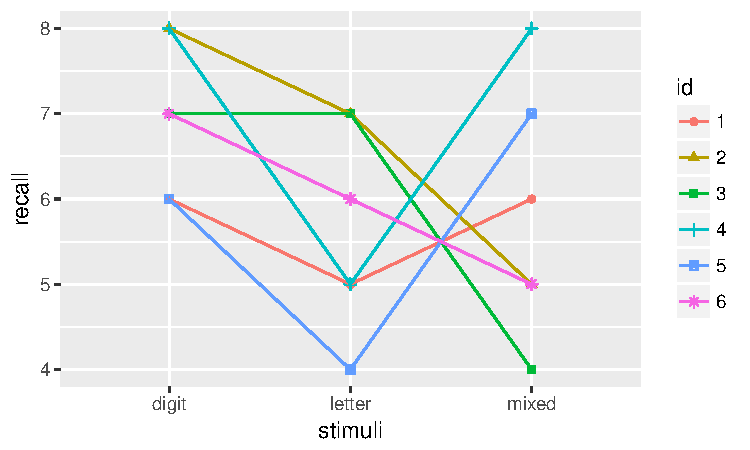
\includegraphics{Unit_5_assignment_KEY_R__spr18__files/figure-latex/unnamed-chunk-23-1} \end{center}

\textbf{Means Plots (raw data)}

\begin{center}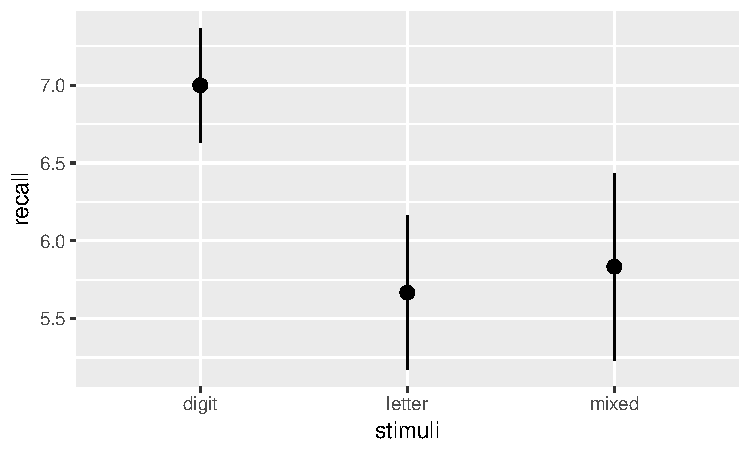
\includegraphics{Unit_5_assignment_KEY_R__spr18__files/figure-latex/unnamed-chunk-24-1} \end{center}

\clearpage

\subsubsection{15B-6a RM ANOVA: with sphericity test and
corrections}\label{b-6a-rm-anova-with-sphericity-test-and-corrections}

\textbf{TEXTBOOK QUESTION:} \emph{(a) Perform an RM ANOVA. Is your
calculated F value significant at the .05 level?}

\textbf{DIRECTIONS:} Perform a Repeated Measures ANOVA for recall under
the three stimuli to determine if the type of stimuli has an effect.
Save it as the name \texttt{fit\_memory} and then use the
\texttt{summary()} function display additional output.

\begin{Shaded}
\begin{Highlighting}[]
\CommentTok{# RM ANOVA: Mauchle Tests for Sphericity and Corrections applied}
\NormalTok{fit_memory <-}\StringTok{ }\NormalTok{memory_long }\OperatorTok\StringTok{ }
\StringTok{  }\NormalTok{afex}\OperatorTok{::}\KeywordTok{aov_4}\NormalTok{(recall }\OperatorTok{~}\StringTok{ }\DecValTok{1} \OperatorTok{+}\StringTok{ }\NormalTok{(stimuli}\OperatorTok{|}\NormalTok{id),}
              \DataTypeTok{data =}\NormalTok{ .) }

\KeywordTok{summary}\NormalTok{(fit_memory)}
\end{Highlighting}
\end{Shaded}

\begin{verbatim}

Univariate Type III Repeated-Measures ANOVA Assuming Sphericity

                SS num Df Error SS den Df        F    Pr(>F)    
(Intercept) 684.50      1    4.500      5 760.5556 1.173e-06 ***
stimuli       6.33      2   17.667     10   1.7925    0.2161    
---
Signif. codes:  0 '***' 0.001 '**' 0.01 '*' 0.05 '.' 0.1 ' ' 1


Mauchly Tests for Sphericity

        Test statistic  p-value
stimuli        0.16661 0.027758


Greenhouse-Geisser and Huynh-Feldt Corrections
 for Departure from Sphericity

         GG eps Pr(>F[GG])
stimuli 0.54544     0.2368

          HF eps Pr(>F[HF])
stimuli 0.581363  0.2355551
\end{verbatim}

\clearpage

\subsubsection{15B-6b RM ANOVA: GG corretion for lack of
sphericity}\label{b-6b-rm-anova-gg-corretion-for-lack-of-sphericity}

\textbf{TEXTBOOK QUESTION:} \emph{(b) Would your conclusion in part a
change if you could not assume that sphericity exists in the population
underlying this experiment? Explain. (c) Based on the graph you drew of
these data for Exercise 15A2, would you say that the RM ANOVA is
appropriate for these data? Explain.}

\textbf{DIRECTIONS:} Run the name of the model \texttt{fit\_memory}
alone to extract the adjusted degrees of freedom and F-test. The
sums-of-squares for the corrected test are the same as for the
uncorrected you just did.

\begin{Shaded}
\begin{Highlighting}[]
\CommentTok{# RM ANOVA: GG correction for lack of sphericity}
\NormalTok{fit_memory }
\end{Highlighting}
\end{Shaded}

\begin{verbatim}
Anova Table (Type 3 tests)

Response: recall
   Effect         df  MSE    F ges p.value
1 stimuli 1.09, 5.45 3.24 1.79 .22     .24
---
Signif. codes:  0 '***' 0.001 '**' 0.01 '*' 0.05 '+' 0.1 ' ' 1

Sphericity correction method: GG 
\end{verbatim}

\clearpage

\subsubsection{15B-6d RM ANOVA: post-hoc with Fisher's LDS
correction}\label{b-6d-rm-anova-post-hoc-with-fishers-lds-correction}

\textbf{TEXTBOOK QUESTION:} \emph{(d) Test all the possible pairs of
means with separate matched t tests (or two-group RM ANOVAs) at the .01
level.}

\textbf{DIRECTIONS:} Conduct all possible post hoc pairwise tests on
\texttt{fit\_audience} using Fisher's LSD.

\begin{Shaded}
\begin{Highlighting}[]
\CommentTok{# RM ANOVA: post hoc all pairwise tests with Fisher's LSD correction}
\NormalTok{fit_memory }\OperatorTok\StringTok{ }
\StringTok{  }\NormalTok{emmeans}\OperatorTok{::}\KeywordTok{emmeans}\NormalTok{(}\OperatorTok{~}\StringTok{ }\NormalTok{stimuli) }\OperatorTok\StringTok{ }
\StringTok{  }\KeywordTok{pairs}\NormalTok{(}\DataTypeTok{correction =} \StringTok{"none"}\NormalTok{)}
\end{Highlighting}
\end{Shaded}

\begin{verbatim}
 contrast         estimate       SE df t.ratio p.value
 digit - letter  1.3333333 0.767391 10   1.737  0.2394
 digit - mixed   1.1666667 0.767391 10   1.520  0.3229
 letter - mixed -0.1666667 0.767391 10  -0.217  0.9744

P value adjustment: tukey method for comparing a family of 3 estimates 
\end{verbatim}

\begin{center}\rule{0.5\linewidth}{\linethickness}\end{center}

\textbf{Means Plot (model based)}

\textbf{DIRECTIONS:} Construct a means plot of \texttt{fit\_audience}
using \texttt{emmeans::emmip(\textasciitilde{}\ RM\_var)} to help
interpret the direction of any significant differences.

\begin{Shaded}
\begin{Highlighting}[]
\CommentTok{# RM ANOVA: means plot}
\NormalTok{memory_long }\OperatorTok\StringTok{ }
\StringTok{  }\NormalTok{afex}\OperatorTok{::}\KeywordTok{aov_4}\NormalTok{(recall }\OperatorTok{~}\StringTok{ }\DecValTok{1} \OperatorTok{+}\StringTok{ }\NormalTok{(stimuli}\OperatorTok{|}\NormalTok{id),}
              \DataTypeTok{data =}\NormalTok{ .)  }\OperatorTok\StringTok{ }
\StringTok{  }\NormalTok{emmeans}\OperatorTok{::}\KeywordTok{emmip}\NormalTok{(}\OperatorTok{~}\StringTok{ }\NormalTok{stimuli)}
\end{Highlighting}
\end{Shaded}

\begin{center}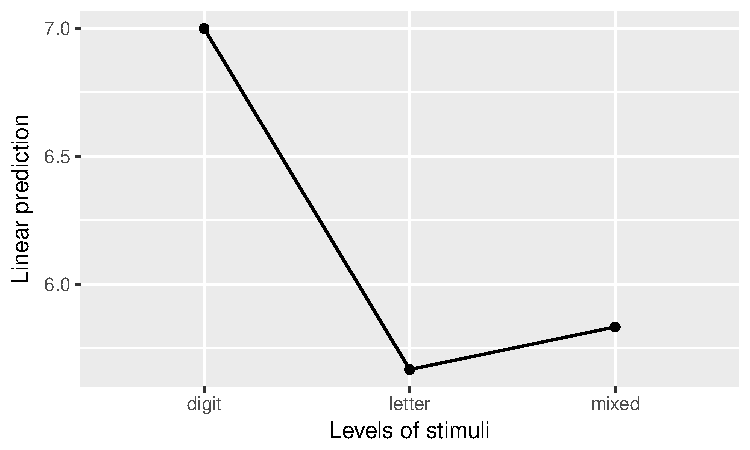
\includegraphics{Unit_5_assignment_KEY_R__spr18__files/figure-latex/unnamed-chunk-28-1} \end{center}

\clearpage

\subsection{\texorpdfstring{\texttt{ihno\_clean} - Repeated Measures
Design: Effect of Time (expereiment) on Anxiety levels (performed
INDEPENDENTLY by
GENDER)}{ihno\_clean - Repeated Measures Design: Effect of Time (expereiment) on Anxiety levels (performed INDEPENDENTLY by GENDER)}}\label{ihno_clean---repeated-measures-design-effect-of-time-expereiment-on-anxiety-levels-performed-independently-by-gender}

\subsubsection{15C-1a RM ANOVA (twice): with sphericity test and
corrections}\label{c-1a-rm-anova-twice-with-sphericity-test-and-corrections}

\textbf{TEXTBOOK QUESTION:} \emph{(a) Use Split File to perform separate
RM ANOVAs for men and women to test for a significant change in anxiety
level over time (baseline, prequiz, and postquiz). Use Options to
request pairwise tests. Write up the results in APA style.}

\begin{Shaded}
\begin{Highlighting}[]
\NormalTok{ihno_clean }\OperatorTok\StringTok{ }
\StringTok{  }\NormalTok{dplyr}\OperatorTok{::}\KeywordTok{select}\NormalTok{(sub_num, anx_base, anx_pre, anx_post) }\OperatorTok\StringTok{ }
\StringTok{  }\KeywordTok{head}\NormalTok{(}\DataTypeTok{n =} \DecValTok{4}\NormalTok{)}
\end{Highlighting}
\end{Shaded}

\begin{verbatim}
# A tibble: 4 x 4
  sub_num anx_base anx_pre anx_post
    <dbl>    <dbl>   <dbl>    <dbl>
1    1.00     17.0    22.0     20.0
2    2.00     17.0    19.0     16.0
3    3.00     19.0    14.0     15.0
4    4.00     19.0    13.0     16.0
\end{verbatim}

Restructure from wide to long format:

\begin{Shaded}
\begin{Highlighting}[]
\CommentTok{#Restructure: wide-to-long}
\NormalTok{ihno_anx_long <-}\StringTok{ }\NormalTok{ihno_clean }\OperatorTok\StringTok{ }
\StringTok{  }\NormalTok{tidyr}\OperatorTok{::}\KeywordTok{gather}\NormalTok{(}\DataTypeTok{key =}\NormalTok{ variable,}
                \DataTypeTok{value =}\NormalTok{ anxiety,}
\NormalTok{                anx_base, anx_pre, anx_post) }\OperatorTok\StringTok{ }
\StringTok{  }\NormalTok{dplyr}\OperatorTok{::}\KeywordTok{mutate}\NormalTok{(}\DataTypeTok{time =} \KeywordTok{case_when}\NormalTok{(variable }\OperatorTok{==}\StringTok{ "anx_base"} \OperatorTok{~}\StringTok{ "baseline"}\NormalTok{,}
\NormalTok{                                 variable }\OperatorTok{==}\StringTok{ "anx_pre"}  \OperatorTok{~}\StringTok{ "pre-quiz"}\NormalTok{,}
\NormalTok{                                 variable }\OperatorTok{==}\StringTok{ "anx_post"} \OperatorTok{~}\StringTok{ "post-quiz"}\NormalTok{) }\OperatorTok\StringTok{ }
\StringTok{                  }\KeywordTok{factor}\NormalTok{(}\DataTypeTok{levels =} \KeywordTok{c}\NormalTok{(}\StringTok{"baseline"}\NormalTok{, }\StringTok{"pre-quiz"}\NormalTok{, }\StringTok{"post-quiz"}\NormalTok{))) }\OperatorTok\StringTok{ }
\StringTok{  }\NormalTok{dplyr}\OperatorTok{::}\KeywordTok{arrange}\NormalTok{(sub_num, time)}
\end{Highlighting}
\end{Shaded}

\begin{Shaded}
\begin{Highlighting}[]
\NormalTok{ihno_anx_long }\OperatorTok\StringTok{ }
\StringTok{  }\NormalTok{dplyr}\OperatorTok{::}\KeywordTok{select}\NormalTok{(sub_num, time, anxiety) }\OperatorTok\StringTok{ }
\StringTok{  }\KeywordTok{head}\NormalTok{(}\DataTypeTok{n =} \DecValTok{12}\NormalTok{)}
\end{Highlighting}
\end{Shaded}

\begin{verbatim}
# A tibble: 12 x 3
   sub_num time      anxiety
     <dbl> <fct>       <dbl>
 1    1.00 baseline     17.0
 2    1.00 pre-quiz     22.0
 3    1.00 post-quiz    20.0
 4    2.00 baseline     17.0
 5    2.00 pre-quiz     19.0
 6    2.00 post-quiz    16.0
 7    3.00 baseline     19.0
 8    3.00 pre-quiz     14.0
 9    3.00 post-quiz    15.0
10    4.00 baseline     19.0
11    4.00 pre-quiz     13.0
12    4.00 post-quiz    16.0
\end{verbatim}

\clearpage

\textbf{RESTRICT to just FEMALES}

\textbf{DIRECTIONS:} Perform a Repeated Measures ANOVA for anxiety at
all three time points to determine if the experiment had an effect. Make
sure to preceed teh ANOVA with a \texttt{dplyr::filter()} step to
restrict to just \texttt{genderF\ ==\ "Female}. Save it as the name
\texttt{fit\_anx\_female} and then use the \texttt{summary()} function
display additional output.

\begin{Shaded}
\begin{Highlighting}[]
\CommentTok{# RM ANOVA: Mauchle Tests for Sphericity with and without corrections applied}
\NormalTok{fit_anx_female <-}\StringTok{ }\NormalTok{ihno_anx_long }\OperatorTok\StringTok{ }
\StringTok{  }\NormalTok{dplyr}\OperatorTok{::}\KeywordTok{filter}\NormalTok{(genderF }\OperatorTok{==}\StringTok{ "Female"}\NormalTok{) }\OperatorTok\StringTok{ }
\StringTok{  }\NormalTok{afex}\OperatorTok{::}\KeywordTok{aov_4}\NormalTok{(anxiety }\OperatorTok{~}\StringTok{ }\DecValTok{1} \OperatorTok{+}\StringTok{ }\NormalTok{(time}\OperatorTok{|}\NormalTok{sub_num),}
              \DataTypeTok{data =}\NormalTok{ .)}

\KeywordTok{summary}\NormalTok{(fit_anx_female)}
\end{Highlighting}
\end{Shaded}

\begin{verbatim}

Univariate Type III Repeated-Measures ANOVA Assuming Sphericity

               SS num Df Error SS den Df        F  Pr(>F)    
(Intercept) 69928      1   4162.9     56 940.6912 < 2e-16 ***
time           87      2   1213.3    112   4.0313 0.02039 *  
---
Signif. codes:  0 '***' 0.001 '**' 0.01 '*' 0.05 '.' 0.1 ' ' 1


Mauchly Tests for Sphericity

     Test statistic   p-value
time        0.81837 0.0040379


Greenhouse-Geisser and Huynh-Feldt Corrections
 for Departure from Sphericity

      GG eps Pr(>F[GG])  
time 0.84629    0.02681 *
---
Signif. codes:  0 '***' 0.001 '**' 0.01 '*' 0.05 '.' 0.1 ' ' 1

        HF eps Pr(>F[HF])
time 0.8698362 0.02571023
\end{verbatim}

\clearpage

\textbf{DIRECTIONS:} If, and only if, the omnibus F test yielded
evidence of at least one time point having a different average anxiety
FOR WOMEN, follow up with post hoc pairs tests based on the ANOVA model.

\begin{Shaded}
\begin{Highlighting}[]
\CommentTok{# RM ANOVA: post hoc all pairwise tests with Fisher's LSD correction}
\NormalTok{fit_anx_female }\OperatorTok\StringTok{ }
\StringTok{  }\NormalTok{emmeans}\OperatorTok{::}\KeywordTok{emmeans}\NormalTok{(}\OperatorTok{~}\StringTok{ }\NormalTok{time) }\OperatorTok
\StringTok{  }\KeywordTok{pairs}\NormalTok{(}\DataTypeTok{adjust =} \StringTok{"none"}\NormalTok{)}
\end{Highlighting}
\end{Shaded}

\begin{verbatim}
 contrast               estimate        SE  df t.ratio p.value
 baseline - pre.quiz  -1.3333333 0.6165333 112  -2.163  0.0327
 baseline - post.quiz -1.6491228 0.6165333 112  -2.675  0.0086
 pre.quiz - post.quiz -0.3157895 0.6165333 112  -0.512  0.6095
\end{verbatim}

\begin{center}\rule{0.5\linewidth}{\linethickness}\end{center}

\textbf{Means Plot (model based)}

\textbf{DIRECTIONS:} If, and only if, the omnibus F test yielded
evidence of at least one time point having a different average anxiety
FOR WOMEN construct a means plot of \texttt{fit\_audience} using
\texttt{emmeans::emmip(\textasciitilde{}\ RM\_var)} to help interpret
the direction of any significant differences.

\begin{Shaded}
\begin{Highlighting}[]
\CommentTok{# Means Plot: model based}
\NormalTok{fit_anx_female }\OperatorTok\StringTok{ }
\StringTok{  }\NormalTok{emmeans}\OperatorTok{::}\KeywordTok{emmip}\NormalTok{(}\OperatorTok{~}\StringTok{ }\NormalTok{time)}
\end{Highlighting}
\end{Shaded}

\begin{center}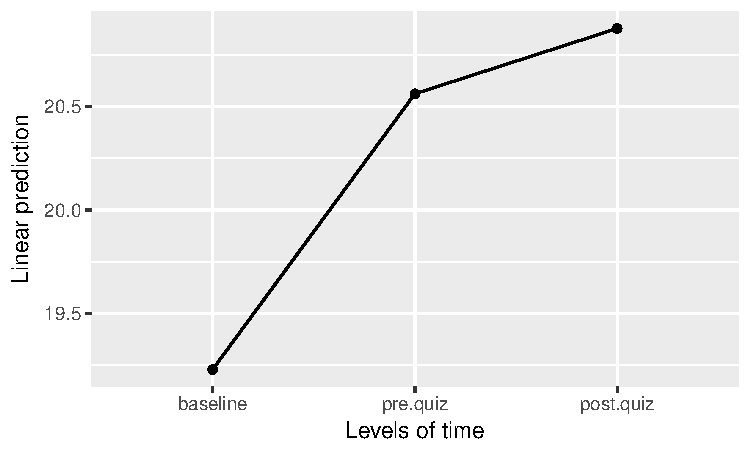
\includegraphics{Unit_5_assignment_KEY_R__spr18__files/figure-latex/unnamed-chunk-34-1} \end{center}

\clearpage

\textbf{RESTRICT to just MALES}

\textbf{DIRECTIONS:} Perform a Repeated Measures ANOVA for anxiety at
all three time points to determine if the experiment had an effect. Make
sure to preceed teh ANOVA with a \texttt{dplyr::filter()} step to
restrict to just \texttt{genderF\ ==\ "Male}. Save it as the name
\texttt{fit\_anx\_male} and then use the \texttt{summary()} function
display additional output.

\begin{Shaded}
\begin{Highlighting}[]
\CommentTok{# RM ANOVA: Mauchle Tests for Sphericity with and without corrections applied}
\NormalTok{fit_anx_male <-}\StringTok{  }\NormalTok{ihno_anx_long }\OperatorTok\StringTok{ }
\StringTok{  }\NormalTok{dplyr}\OperatorTok{::}\KeywordTok{filter}\NormalTok{(genderF }\OperatorTok{==}\StringTok{ "Male"}\NormalTok{) }\OperatorTok\StringTok{ }
\StringTok{  }\NormalTok{afex}\OperatorTok{::}\KeywordTok{aov_4}\NormalTok{(anxiety }\OperatorTok{~}\StringTok{ }\DecValTok{1} \OperatorTok{+}\StringTok{ }\NormalTok{(time}\OperatorTok{|}\NormalTok{sub_num),}
              \DataTypeTok{data =}\NormalTok{ .) }

\KeywordTok{summary}\NormalTok{(fit_anx_male)}
\end{Highlighting}
\end{Shaded}

\begin{verbatim}

Univariate Type III Repeated-Measures ANOVA Assuming Sphericity

               SS num Df Error SS den Df         F Pr(>F)    
(Intercept) 40404      1  1549.88     42 1094.9000 <2e-16 ***
time           22      2   777.43     84    1.1835 0.3113    
---
Signif. codes:  0 '***' 0.001 '**' 0.01 '*' 0.05 '.' 0.1 ' ' 1


Mauchly Tests for Sphericity

     Test statistic    p-value
time        0.60308 3.1452e-05


Greenhouse-Geisser and Huynh-Feldt Corrections
 for Departure from Sphericity

      GG eps Pr(>F[GG])
time 0.71586     0.2999

       HF eps Pr(>F[HF])
time 0.734119  0.3009149
\end{verbatim}

\clearpage

\textbf{DIRECTIONS:} If, and only if, the omnibus F test yielded
evidence of at least one time point having a different average anxiety
FOR MEN, follow up with post hoc pairs tests based on the ANOVA model.

\begin{Shaded}
\begin{Highlighting}[]
\CommentTok{# RM ANOVA: post hoc all pairwise tests with Fisher's LSD correction}
\end{Highlighting}
\end{Shaded}

\begin{center}\rule{0.5\linewidth}{\linethickness}\end{center}

\textbf{Means Plot (model based)}

\textbf{DIRECTIONS:} If, and only if, the omnibus F test yielded
evidence of at least one time point having a different average anxiety
FOR MEN, construct a means plot of \texttt{fit\_audience} using
\texttt{emmeans::emmip(\textasciitilde{}\ RM\_var)} to help interpret
the direction of any significant differences.

\begin{Shaded}
\begin{Highlighting}[]
\CommentTok{# Means Plot: model based}
\end{Highlighting}
\end{Shaded}

\clearpage

\subsubsection{15C-1b Paired t-Tests: choose 2 at a
time}\label{c-1b-paired-t-tests-choose-2-at-a-time}

\textbf{TEXTBOOK QUESTION:} \emph{(b) Using ANALYZE/Compare Means ,
perform matched t tests for each pair of RM levels, and then compare
these p values to those produced in the Pairwise Comparisons results box
of the RM ANOVA.}

\textbf{DIRECTIONS:} If, and only if, the omnibus F test yielded
evidence of at least one time point having a different average anxiety
FOR WOMEN, follow up with post hoc pairs tests NOT based on the ANOVA
model. Instead, increase your \texttt{dplyr::filter()} to include
requiring only 2 of the 3 time points (eg.
\texttt{time\ \%in\%\ c("baseline",\ "pre-quiz")}). You will have to do
this 3 times, as there are three ways to choose a pair from three
options.

\begin{Shaded}
\begin{Highlighting}[]
\CommentTok{# Paired T-test: filter - women & baseline/pre-quiz}
\NormalTok{ihno_anx_long }\OperatorTok\StringTok{ }
\StringTok{  }\NormalTok{dplyr}\OperatorTok{::}\KeywordTok{filter}\NormalTok{(genderF }\OperatorTok{==}\StringTok{ "Female"} \OperatorTok{&}\StringTok{ }\NormalTok{time }\OperatorTok\StringTok{ }\KeywordTok{c}\NormalTok{(}\StringTok{"baseline"}\NormalTok{, }\StringTok{"pre-quiz"}\NormalTok{)) }\OperatorTok\StringTok{ }
\StringTok{  }\KeywordTok{t.test}\NormalTok{(anxiety }\OperatorTok{~}\StringTok{ }\NormalTok{time,}
         \DataTypeTok{data =}\NormalTok{ .,}
         \DataTypeTok{paired =} \OtherTok{TRUE}\NormalTok{)}
\end{Highlighting}
\end{Shaded}

\begin{verbatim}

    Paired t-test

data:  anxiety by time
t = -1.8192, df = 56, p-value = 0.07423
alternative hypothesis: true difference in means is not equal to 0
95 percent confidence interval:
 -2.8015547  0.1348881
sample estimates:
mean of the differences 
              -1.333333 
\end{verbatim}

\begin{Shaded}
\begin{Highlighting}[]
\CommentTok{# Paired T-test: filter - women & baseline or post-quiz}
\NormalTok{ihno_anx_long }\OperatorTok\StringTok{ }
\StringTok{  }\NormalTok{dplyr}\OperatorTok{::}\KeywordTok{filter}\NormalTok{(genderF }\OperatorTok{==}\StringTok{ "Female"} \OperatorTok{&}\StringTok{ }\NormalTok{time }\OperatorTok\StringTok{ }\KeywordTok{c}\NormalTok{(}\StringTok{"baseline"}\NormalTok{, }\StringTok{"post-quiz"}\NormalTok{)) }\OperatorTok\StringTok{ }
\StringTok{  }\KeywordTok{t.test}\NormalTok{(anxiety }\OperatorTok{~}\StringTok{ }\NormalTok{time,}
         \DataTypeTok{data =}\NormalTok{ .,}
         \DataTypeTok{paired =} \OtherTok{TRUE}\NormalTok{)}
\end{Highlighting}
\end{Shaded}

\begin{verbatim}

    Paired t-test

data:  anxiety by time
t = -3.1902, df = 56, p-value = 0.00233
alternative hypothesis: true difference in means is not equal to 0
95 percent confidence interval:
 -2.6846744 -0.6135712
sample estimates:
mean of the differences 
              -1.649123 
\end{verbatim}

\begin{Shaded}
\begin{Highlighting}[]
\CommentTok{# Paired T-test: filter - women & pre-quiz/post-quiz}
\NormalTok{ihno_anx_long }\OperatorTok\StringTok{ }
\StringTok{  }\NormalTok{dplyr}\OperatorTok{::}\KeywordTok{filter}\NormalTok{(genderF }\OperatorTok{==}\StringTok{ "Female"} \OperatorTok{&}\StringTok{ }\NormalTok{time }\OperatorTok\StringTok{ }\KeywordTok{c}\NormalTok{(}\StringTok{"pre-quiz"}\NormalTok{, }\StringTok{"post-quiz"}\NormalTok{)) }\OperatorTok\StringTok{ }
\StringTok{  }\KeywordTok{t.test}\NormalTok{(anxiety }\OperatorTok{~}\StringTok{ }\NormalTok{time,}
         \DataTypeTok{data =}\NormalTok{ .,}
         \DataTypeTok{paired =} \OtherTok{TRUE}\NormalTok{) }
\end{Highlighting}
\end{Shaded}

\begin{verbatim}

    Paired t-test

data:  anxiety by time
t = -0.54484, df = 56, p-value = 0.588
alternative hypothesis: true difference in means is not equal to 0
95 percent confidence interval:
 -1.4768719  0.8452929
sample estimates:
mean of the differences 
             -0.3157895 
\end{verbatim}

\clearpage

\textbf{DIRECTIONS:} If, and only if, the omnibus F test yielded
evidence of at least one time point having a different average anxiety
FOR MEN, follow up with post hoc pairs tests NOT based on the ANOVA
model. Instead, increase your \texttt{dplyr::filter()} to include
requiring only 2 of the 3 time points (eg.
\texttt{time\ \%in\%\ c("baseline",\ "pre-quiz")}). You will have to do
this 3 times, as there are three ways to choose a pair from three
options.

\begin{Shaded}
\begin{Highlighting}[]
\CommentTok{# Paired T-test: filter - men & baseline/pre-quiz}
\end{Highlighting}
\end{Shaded}

\begin{Shaded}
\begin{Highlighting}[]
\CommentTok{# Paired T-test: filter - men & baseline or post-quiz}
\end{Highlighting}
\end{Shaded}

\begin{Shaded}
\begin{Highlighting}[]
\CommentTok{# Paired T-test: filter - men & pre-quiz/post-quiz}
\end{Highlighting}
\end{Shaded}

\clearpage

\subsection{\texorpdfstring{\texttt{ihno\_clean} - Repeated Measures
Design: Effect of experiemnt (with vs without the experimental item) on
Stat
Quiz}{ihno\_clean - Repeated Measures Design: Effect of experiemnt (with vs without the experimental item) on Stat Quiz}}\label{ihno_clean---repeated-measures-design-effect-of-experiemnt-with-vs-without-the-experimental-item-on-stat-quiz}

\subsubsection{15C-3 RM ANOVA vs.~Paired t-test: only 2
groups}\label{c-3-rm-anova-vs.paired-t-test-only-2-groups}

\textbf{TEXTBOOK QUESTION:} \emph{Perform an RM ANOVA to determine
whether there is a significant difference in mean scores between the
experimental stats quiz and the regular stats quiz. Compare this F ratio
with the matched t value you obtained from computer exercise \#3 in
Chapter 11.}

Restructure: wide-to-long

\begin{Shaded}
\begin{Highlighting}[]
\NormalTok{ihno_clean }\OperatorTok\StringTok{ }
\StringTok{  }\NormalTok{dplyr}\OperatorTok{::}\KeywordTok{select}\NormalTok{(sub_num, statquiz, exp_sqz) }\OperatorTok\StringTok{ }
\StringTok{  }\KeywordTok{head}\NormalTok{(}\DataTypeTok{n =} \DecValTok{5}\NormalTok{)}
\end{Highlighting}
\end{Shaded}

\begin{verbatim}
# A tibble: 5 x 3
  sub_num statquiz exp_sqz
    <dbl>    <dbl>   <dbl>
1    1.00     6.00    7.00
2    2.00     9.00   11.0 
3    3.00     8.00    8.00
4    4.00     7.00    8.00
5    5.00     6.00    6.00
\end{verbatim}

\begin{Shaded}
\begin{Highlighting}[]
\NormalTok{ihno_statquiz_long <-}\StringTok{ }\NormalTok{ihno_clean }\OperatorTok\StringTok{ }
\StringTok{  }\NormalTok{tidyr}\OperatorTok{::}\KeywordTok{gather}\NormalTok{(}\DataTypeTok{key =}\NormalTok{ variable,}
                \DataTypeTok{value =}\NormalTok{ s_quiz,}
\NormalTok{                statquiz, exp_sqz) }\OperatorTok\StringTok{ }
\StringTok{  }\NormalTok{dplyr}\OperatorTok{::}\KeywordTok{mutate}\NormalTok{(}\DataTypeTok{time =} \KeywordTok{case_when}\NormalTok{(variable }\OperatorTok{==}\StringTok{ "statquiz"} \OperatorTok{~}\StringTok{ "background"}\NormalTok{,}
\NormalTok{                                 variable }\OperatorTok{==}\StringTok{ "exp_sqz"}  \OperatorTok{~}\StringTok{ "experimental"}\NormalTok{) }\OperatorTok\StringTok{ }
\StringTok{                  }\KeywordTok{factor}\NormalTok{()) }\OperatorTok\StringTok{ }
\StringTok{  }\NormalTok{dplyr}\OperatorTok{::}\KeywordTok{arrange}\NormalTok{(sub_num, time)}
\end{Highlighting}
\end{Shaded}

\begin{Shaded}
\begin{Highlighting}[]
\NormalTok{ihno_statquiz_long }\OperatorTok\StringTok{ }
\StringTok{  }\NormalTok{dplyr}\OperatorTok{::}\KeywordTok{select}\NormalTok{(sub_num, time, s_quiz) }\OperatorTok\StringTok{ }
\StringTok{  }\KeywordTok{head}\NormalTok{(}\DataTypeTok{n =} \DecValTok{10}\NormalTok{)}
\end{Highlighting}
\end{Shaded}

\begin{verbatim}
# A tibble: 10 x 3
   sub_num time         s_quiz
     <dbl> <fct>         <dbl>
 1    1.00 background     6.00
 2    1.00 experimental   7.00
 3    2.00 background     9.00
 4    2.00 experimental  11.0 
 5    3.00 background     8.00
 6    3.00 experimental   8.00
 7    4.00 background     7.00
 8    4.00 experimental   8.00
 9    5.00 background     6.00
10    5.00 experimental   6.00
\end{verbatim}

\clearpage

\textbf{DIRECTIONS:} Perform a Repeated Measures ANOVA for recall under
the three stimuli to determine if the type of stimuli has an effect. Do
not save this model as a name; just run it without nameing/saving it.

\begin{quote}
NOTE: When the measure is only repeated twice, sphericity can not be
violated, so no such test are performed.
\end{quote}

\begin{Shaded}
\begin{Highlighting}[]
\CommentTok{# RM ANOVA: no correction for lack of sphericity }
\NormalTok{ihno_statquiz_long }\OperatorTok\StringTok{ }
\StringTok{  }\NormalTok{afex}\OperatorTok{::}\KeywordTok{aov_4}\NormalTok{(s_quiz }\OperatorTok{~}\StringTok{ }\DecValTok{1} \OperatorTok{+}\StringTok{ }\NormalTok{(time}\OperatorTok{|}\NormalTok{sub_num),}
              \DataTypeTok{data =}\NormalTok{ .)}
\end{Highlighting}
\end{Shaded}

\begin{verbatim}
Anova Table (Type 3 tests)

Response: s_quiz
  Effect    df  MSE    F    ges p.value
1   time 1, 99 1.11 0.04 <.0001     .84
---
Signif. codes:  0 '***' 0.001 '**' 0.01 '*' 0.05 '+' 0.1 ' ' 1
\end{verbatim}

\begin{center}\rule{0.5\linewidth}{\linethickness}\end{center}

\textbf{DIRECTIONS:} Alternatively, since there are only two measures,
you can run this same analysis as a paired t.test, using
\texttt{t.test()}. Make sure you include \texttt{paired\ =\ TRUE}.

\begin{Shaded}
\begin{Highlighting}[]
\CommentTok{# Matched t-test: paired = TRUE}
\NormalTok{ihno_statquiz_long }\OperatorTok\StringTok{ }
\StringTok{  }\KeywordTok{t.test}\NormalTok{(s_quiz }\OperatorTok{~}\StringTok{ }\NormalTok{time,}
         \DataTypeTok{data =}\NormalTok{ .,}
         \DataTypeTok{paired =} \OtherTok{TRUE}\NormalTok{)}
\end{Highlighting}
\end{Shaded}

\begin{verbatim}

    Paired t-test

data:  s_quiz by time
t = 0.20175, df = 99, p-value = 0.8405
alternative hypothesis: true difference in means is not equal to 0
95 percent confidence interval:
 -0.2650559  0.3250559
sample estimates:
mean of the differences 
                   0.03 
\end{verbatim}

\clearpage

\section{Chapter 16: Mixed Design
ANOVA}\label{chapter-16-mixed-design-anova}

\subsection{\texorpdfstring{Tutorial - Fitting Mixed Design ANOVA Models
with
\texttt{afex::aov\_4()}}{Tutorial - Fitting Mixed Design ANOVA Models with afex::aov\_4()}}\label{tutorial---fitting-mixed-design-anova-models-with-afexaov_4}

The \texttt{aov\_4()} function from the \texttt{afex} package fits ANOVA
models (oneway, two-way, repeated measures, and mixed design). It needs
at least two arguments:

\begin{enumerate}
\def\labelenumi{\arabic{enumi}.}
\item
  formula:
  \texttt{continuous\_var\ \textasciitilde{}\ group\_var\ +\ (RM\_var\textbar{}id\_var)}
  \emph{one observation per subject for each level of the
  \texttt{RMvar}, so each \texttt{id\_var} has multiple lines for each
  subject, each subject can only belong to exactly one group./}
\item
  dataset: \texttt{data\ =\ .} \emph{we use the period to signify that
  the datset is being piped from above}
\end{enumerate}

Here is an outline of what your syntax should look like when you
\textbf{fit and save a Mixed ANOVA}. Of course you will replace the
dataset name and the variable names, as well as the name you are saving
it as.

\begin{quote}
\textbf{NOTE:} The \texttt{aov\_4()} function works on data in LONG
format only. Each observation needs to be on its one line or row with
seperate variables for the group membership (categorical factor or
\texttt{fct}) and the continuous measurement (numberic or \texttt{dbl}).
\end{quote}

\begin{Shaded}
\begin{Highlighting}[]
\CommentTok{# RM ANOVA: fit and save}
\NormalTok{aov_name <-}\StringTok{ }\NormalTok{data_name }\OperatorTok\StringTok{ }
\StringTok{  }\NormalTok{afex}\OperatorTok{::}\KeywordTok{aov_4}\NormalTok{(continuous_var }\OperatorTok{~}\StringTok{ }\NormalTok{group_var }\OperatorTok{+}\StringTok{ }\NormalTok{(RM_var}\OperatorTok{|}\NormalTok{id_var),}
              \DataTypeTok{data =}\NormalTok{ .)}
\end{Highlighting}
\end{Shaded}

\clearpage

\subsection{\texorpdfstring{\texttt{tasks\_wide} - Repeated Measures and
Assigned Group Design: Differential Effect of Music on Production, by
Task
Type}{tasks\_wide - Repeated Measures and Assigned Group Design: Differential Effect of Music on Production, by Task Type}}\label{tasks_wide---repeated-measures-and-assigned-group-design-differential-effect-of-music-on-production-by-task-type}

\textbf{TEXTBOOK QUESTION:} \emph{In Exercise 15B1, subjects performed a
clerical task under three noise conditions. Now suppose a new group of
subjects is added to study the effects of the same three conditions on
the performance of a simpler, more mechanical task. The data from
Exercise 15B1 follow, along with the data for the mechanical task.}

\begin{verbatim}
  clerical_background clerical_popular clerical_metal
1                  10               12              8
2                   7                9              4
3                  13               15              9
4                  18               12              6
5                   6                8              3
  mechanical_background mechanical_popular mechanical_metal
1                    15                 18               20
2                    19                 22               23
3                     8                 12               15
4                    10                 10               14
5                    16                 19               19
\end{verbatim}

\begin{center}\rule{0.5\linewidth}{\linethickness}\end{center}

\begin{verbatim}
   id  type_task      noise completed
1   1   clerical background        10
2   2   clerical background         7
3   3   clerical background        13
4   4   clerical background        18
5   5   clerical background         6
6   1   clerical    popular        12
7   2   clerical    popular         9
8   3   clerical    popular        15
9   4   clerical    popular        12
10  5   clerical    popular         8
11  1   clerical      metal         8
12  2   clerical      metal         4
13  3   clerical      metal         9
14  4   clerical      metal         6
15  5   clerical      metal         3
16  6 mechanical background        15
17  7 mechanical background        19
18  8 mechanical background         8
19  9 mechanical background        10
20 10 mechanical background        16
\end{verbatim}

\clearpage

\textbf{Summary Statistics}

\begin{longtable}[]{@{}cccc@{}}
\toprule
\begin{minipage}[b]{0.16\columnwidth}\centering\strut
type\_task\strut
\end{minipage} & \begin{minipage}[b]{0.17\columnwidth}\centering\strut
background\strut
\end{minipage} & \begin{minipage}[b]{0.16\columnwidth}\centering\strut
metal\strut
\end{minipage} & \begin{minipage}[b]{0.16\columnwidth}\centering\strut
popular\strut
\end{minipage}\tabularnewline
\midrule
\endhead
\begin{minipage}[t]{0.16\columnwidth}\centering\strut
clerical\strut
\end{minipage} & \begin{minipage}[t]{0.17\columnwidth}\centering\strut
10.8 (4.87)\strut
\end{minipage} & \begin{minipage}[t]{0.16\columnwidth}\centering\strut
6 (2.55)\strut
\end{minipage} & \begin{minipage}[t]{0.16\columnwidth}\centering\strut
11.2 (2.77)\strut
\end{minipage}\tabularnewline
\begin{minipage}[t]{0.16\columnwidth}\centering\strut
mechanical\strut
\end{minipage} & \begin{minipage}[t]{0.17\columnwidth}\centering\strut
13.6 (4.51)\strut
\end{minipage} & \begin{minipage}[t]{0.16\columnwidth}\centering\strut
18.2 (3.7)\strut
\end{minipage} & \begin{minipage}[t]{0.16\columnwidth}\centering\strut
16.2 (5.02)\strut
\end{minipage}\tabularnewline
\bottomrule
\end{longtable}

\textbf{Profile Plots (raw data)}

\begin{center}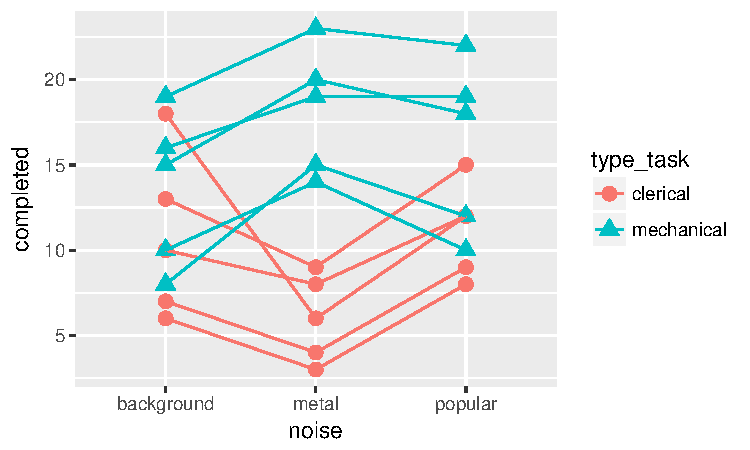
\includegraphics{Unit_5_assignment_KEY_R__spr18__files/figure-latex/unnamed-chunk-52-1} \end{center}

\textbf{Means Plots (raw data)}

\begin{center}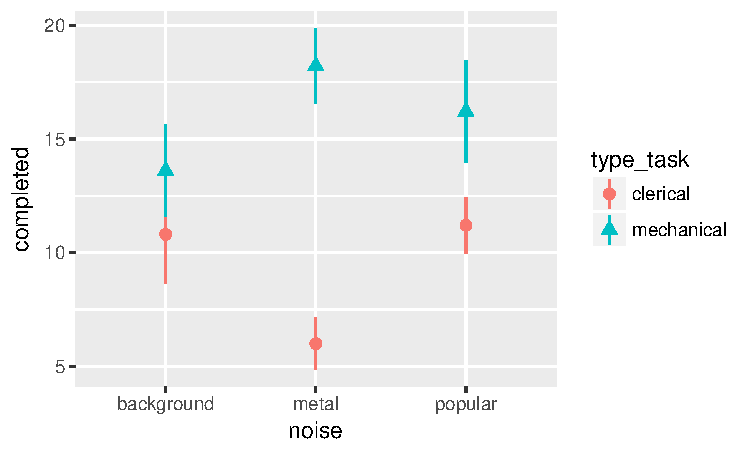
\includegraphics{Unit_5_assignment_KEY_R__spr18__files/figure-latex/unnamed-chunk-53-1} \end{center}

\clearpage

\subsubsection{16B-4a Mixed Design ANOVA: display all Sums-of-Squares
components}\label{b-4a-mixed-design-anova-display-all-sums-of-squares-components}

\textbf{TEXTBOOK QUESTION:} \emph{(a) Perform a mixed-design ANOVA, and
display the results in a summary table.}

\textbf{DIRECTIONS:} Perform a Repeated Measures ANOVA for number of
tasks completed under the four noise conditions to see if there is an
effect and if the effect is different dependtion on the type of task.
Request no correction for violations of sphericity
(\texttt{correction\ =\ "none"}) and both effect sizes
(\texttt{es\ =\ c("ges",\ "pes"}). Make sure to save your model
(\texttt{fit\_tasks}), so that you can add \texttt{\$aov} at the end of
the name to extract all the Sums-of-Squares.

\begin{Shaded}
\begin{Highlighting}[]
\CommentTok{# Mixed ANOVA: display all Sums-of-Squares components}
\NormalTok{fit_tasks <-}\StringTok{ }\NormalTok{tasks_long }\OperatorTok\StringTok{ }
\StringTok{  }\NormalTok{afex}\OperatorTok{::}\KeywordTok{aov_4}\NormalTok{(completed }\OperatorTok{~}\StringTok{ }\NormalTok{type_task }\OperatorTok{+}\StringTok{ }\NormalTok{(noise}\OperatorTok{|}\NormalTok{id),}
              \DataTypeTok{data =}\NormalTok{ .,}
              \DataTypeTok{anova_table =} \KeywordTok{list}\NormalTok{(}\DataTypeTok{correction =} \StringTok{"none"}\NormalTok{,}
                                 \DataTypeTok{es =} \KeywordTok{c}\NormalTok{(}\StringTok{"ges"}\NormalTok{, }\StringTok{"pes"}\NormalTok{))) }

\NormalTok{fit_tasks}\OperatorTok{$}\NormalTok{aov}
\end{Highlighting}
\end{Shaded}

\begin{verbatim}

Call:
aov(formula = formula(paste(dv.escaped, "~", paste(c(between.escaped, 
    within.escaped), collapse = "*"), if (length(within) > 0) paste0("+Error(", 
    id.escaped, "/(", paste(within.escaped, collapse = "*"), 
    "))") else NULL)), data = dat.ret, contrasts = contrasts)

Grand Mean: 12.66667

Stratum 1: id

Terms:
                type_task Residuals
Sum of Squares   333.3333  338.6667
Deg. of Freedom         1         8

Residual standard error: 6.506407
Estimated effects are balanced

Stratum 2: id:noise

Terms:
                    noise type_task:noise Residuals
Sum of Squares   16.06667       120.86667  49.73333
Deg. of Freedom         2               2        16

Residual standard error: 1.763047
Estimated effects may be unbalanced
\end{verbatim}

\clearpage

\subsubsection{16B-4b Mixed Design ANOVA: effect
sizes}\label{b-4b-mixed-design-anova-effect-sizes}

\textbf{TEXTBOOK QUESTION:} \emph{(b) Calculate generalized eta squared
for the main effect of the type-of-task factor. Does this look like a
large effect size? Explain.}

\textbf{DIRECTIONS:} Run the name of the model \texttt{fit\_tasks} alone
to extract the adjusted degrees of freedom and F-test. The
sums-of-squares for the corrected test are the same as for the
uncorrected you just did.

\begin{Shaded}
\begin{Highlighting}[]
\CommentTok{# Mixed ANOVA: name the model was saved as}
\NormalTok{fit_tasks}
\end{Highlighting}
\end{Shaded}

\begin{verbatim}
Anova Table (Type 3 tests)

Response: completed
           Effect    df   MSE         F ges pes p.value
1       type_task  1, 8 42.33    7.87 * .46 .50     .02
2           noise 2, 16  3.11      2.58 .04 .24     .11
3 type_task:noise 2, 16  3.11 19.44 *** .24 .71  <.0001
---
Signif. codes:  0 '***' 0.001 '**' 0.01 '*' 0.05 '+' 0.1 ' ' 1
\end{verbatim}

\begin{center}\rule{0.5\linewidth}{\linethickness}\end{center}

\textbf{Means Plot (model based)}

\textbf{DIRECTIONS:} Construct a means plot of \texttt{fit\_audience}
using \texttt{emmeans::emmip(\textasciitilde{}\ RM\_var)} to help
interpret the direction of any significant differences.

\begin{Shaded}
\begin{Highlighting}[]
\CommentTok{# RM ANOVA: means plot}
\NormalTok{tasks_long }\OperatorTok\StringTok{ }
\StringTok{  }\NormalTok{afex}\OperatorTok{::}\KeywordTok{aov_4}\NormalTok{(completed }\OperatorTok{~}\StringTok{ }\NormalTok{type_task }\OperatorTok{+}\StringTok{ }\NormalTok{(noise}\OperatorTok{|}\NormalTok{id),}
              \DataTypeTok{data =}\NormalTok{ .) }\OperatorTok\StringTok{ }
\StringTok{  }\NormalTok{emmeans}\OperatorTok{::}\KeywordTok{emmip}\NormalTok{(type_task }\OperatorTok{~}\StringTok{ }\NormalTok{noise)}
\end{Highlighting}
\end{Shaded}

\begin{center}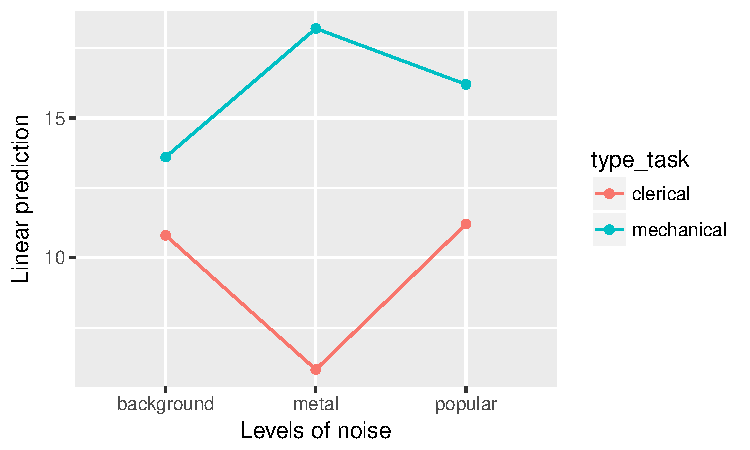
\includegraphics{Unit_5_assignment_KEY_R__spr18__files/figure-latex/unnamed-chunk-56-1} \end{center}

\clearpage

\subsection{\texorpdfstring{\texttt{anograms\_wide} -Repeated Measures
and Assigned Group Design: Effect of Music and Task Type on
Production}{anograms\_wide -Repeated Measures and Assigned Group Design: Effect of Music and Task Type on Production}}\label{anograms_wide--repeated-measures-and-assigned-group-design-effect-of-music-and-task-type-on-production}

\textbf{TEXTBOOK QUESTION:} \emph{Dr.~Jones is investigating various
conditions that affect mental effort- which, in this experiment,
involves solving anagrams. Subjects were randomly assigned to one of
three experimental conditions. Subjects in the first group were told
that they would not be getting feedback on their performance. Subjects
in the second and third groups were told they would get feedback, but
only subjects in the third group were told (erroneously) that anagram
solving was highly correlated with intelligence and creativity
(Dr.~Jones hoped this information would produce ego involvement). The
list of anagrams given to each subject contained a random mix of
problems at four levels of difficulty determined by the number of
letters presented (five, six, seven, or eight). The number of anagrams
correctly solved by each subject in each condition and at each level of
difficulty is given in the following table:}

\begin{Shaded}
\begin{Highlighting}[]
\NormalTok{anograms_wide}
\end{Highlighting}
\end{Shaded}

\begin{verbatim}
  none_5 none_6 none_7 none_8 alone_5 alone_6 alone_7 alone_8 withEgo_5
1      9      6      4      2      19      16      15      12        30
2     10      7      4      3      19      15      11      11        31
3     12      9      7      5      22      20      17      14        34
  withEgo_6 withEgo_7 withEgo_8
1        25        22        21
2        30        27        23
3        32        28        24
\end{verbatim}

\begin{center}\rule{0.5\linewidth}{\linethickness}\end{center}

Restructure from wide to long format:

\begin{verbatim}
   id feedback difficulty correct
1   1     none          5       9
2   2     none          5      10
3   3     none          5      12
4   1     none          6       6
5   2     none          6       7
6   3     none          6       9
7   1     none          7       4
8   2     none          7       4
9   3     none          7       7
10  1     none          8       2
11  2     none          8       3
12  3     none          8       5
13  4    alone          5      19
14  5    alone          5      19
15  6    alone          5      22
16  4    alone          6      16
17  5    alone          6      15
18  6    alone          6      20
19  4    alone          7      15
20  5    alone          7      11
\end{verbatim}

\clearpage

\textbf{Summary Statistics}

\begin{longtable}[]{@{}ccccc@{}}
\toprule
\begin{minipage}[b]{0.13\columnwidth}\centering\strut
feedback\strut
\end{minipage} & \begin{minipage}[b]{0.18\columnwidth}\centering\strut
5\strut
\end{minipage} & \begin{minipage}[b]{0.17\columnwidth}\centering\strut
6\strut
\end{minipage} & \begin{minipage}[b]{0.18\columnwidth}\centering\strut
7\strut
\end{minipage} & \begin{minipage}[b]{0.18\columnwidth}\centering\strut
8\strut
\end{minipage}\tabularnewline
\midrule
\endhead
\begin{minipage}[t]{0.13\columnwidth}\centering\strut
alone\strut
\end{minipage} & \begin{minipage}[t]{0.18\columnwidth}\centering\strut
20 (1.73)\strut
\end{minipage} & \begin{minipage}[t]{0.17\columnwidth}\centering\strut
17 (2.65)\strut
\end{minipage} & \begin{minipage}[t]{0.18\columnwidth}\centering\strut
14.33 (3.06)\strut
\end{minipage} & \begin{minipage}[t]{0.18\columnwidth}\centering\strut
12.33 (1.53)\strut
\end{minipage}\tabularnewline
\begin{minipage}[t]{0.13\columnwidth}\centering\strut
none\strut
\end{minipage} & \begin{minipage}[t]{0.18\columnwidth}\centering\strut
10.33 (1.53)\strut
\end{minipage} & \begin{minipage}[t]{0.17\columnwidth}\centering\strut
7.33 (1.53)\strut
\end{minipage} & \begin{minipage}[t]{0.18\columnwidth}\centering\strut
5 (1.73)\strut
\end{minipage} & \begin{minipage}[t]{0.18\columnwidth}\centering\strut
3.33 (1.53)\strut
\end{minipage}\tabularnewline
\begin{minipage}[t]{0.13\columnwidth}\centering\strut
withEgo\strut
\end{minipage} & \begin{minipage}[t]{0.18\columnwidth}\centering\strut
31.67 (2.08)\strut
\end{minipage} & \begin{minipage}[t]{0.17\columnwidth}\centering\strut
29 (3.61)\strut
\end{minipage} & \begin{minipage}[t]{0.18\columnwidth}\centering\strut
25.67 (3.21)\strut
\end{minipage} & \begin{minipage}[t]{0.18\columnwidth}\centering\strut
22.67 (1.53)\strut
\end{minipage}\tabularnewline
\bottomrule
\end{longtable}

\textbf{Profile Plots (raw data)}

\begin{center}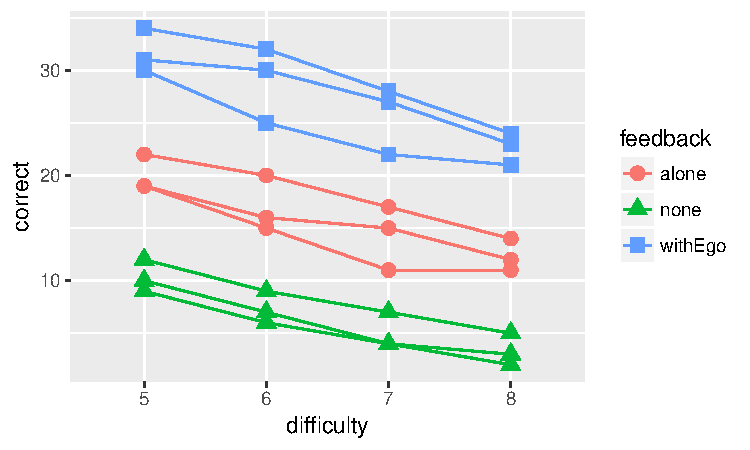
\includegraphics{Unit_5_assignment_KEY_R__spr18__files/figure-latex/unnamed-chunk-60-1} \end{center}

\textbf{Means Plots (raw data)}

\begin{center}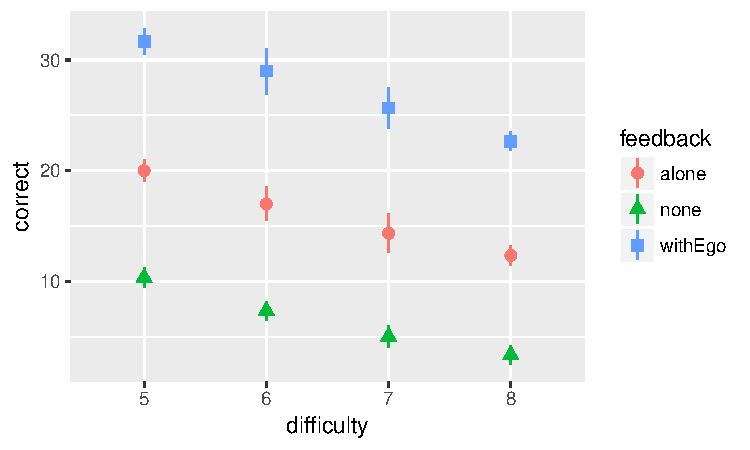
\includegraphics{Unit_5_assignment_KEY_R__spr18__files/figure-latex/unnamed-chunk-61-1} \end{center}

\clearpage

\subsubsection{16B-5b Mixed Design ANOVA: display all Sums-of-Squares
components}\label{b-5b-mixed-design-anova-display-all-sums-of-squares-components}

\textbf{TEXTBOOK QUESTION:} \emph{(b) Perform a mixed analysis of
variance, and display the results in a summary table. Would any of your
conclusions change if you do not assume sphericity? Explain.}

\textbf{DIRECTIONS:} Perform a Repeated Measures ANOVA for number of
tasks completed under the four noise conditions to see if there is an
effect and if the effect is different dependtion on the type of task.
Make sure to save your model (\texttt{fit\_ano}), so that you can add
\texttt{\$aov} at the end of the name to extract all the
Sums-of-Squares.

\begin{Shaded}
\begin{Highlighting}[]
\CommentTok{# Mixed ANOVA: display all Sums-of-Squares components}
\NormalTok{fit_ano <-}\StringTok{ }\NormalTok{anograms_long }\OperatorTok\StringTok{ }
\StringTok{  }\NormalTok{afex}\OperatorTok{::}\KeywordTok{aov_4}\NormalTok{(correct }\OperatorTok{~}\StringTok{ }\NormalTok{feedback }\OperatorTok{+}\StringTok{ }\NormalTok{(difficulty}\OperatorTok{|}\NormalTok{id),}
            \DataTypeTok{data =}\NormalTok{ .) }

\NormalTok{fit_ano}\OperatorTok{$}\NormalTok{aov}
\end{Highlighting}
\end{Shaded}

\begin{verbatim}

Call:
aov(formula = formula(paste(dv.escaped, "~", paste(c(between.escaped, 
    within.escaped), collapse = "*"), if (length(within) > 0) paste0("+Error(", 
    id.escaped, "/(", paste(within.escaped, collapse = "*"), 
    "))") else NULL)), data = dat.ret, contrasts = contrasts)

Grand Mean: 16.55556

Stratum 1: id

Terms:
                 feedback Residuals
Sum of Squares  2590.7222  108.1667
Deg. of Freedom         2         6

Residual standard error: 4.245913
Estimated effects may be unbalanced

Stratum 2: id:difficulty

Terms:
                difficulty feedback:difficulty Residuals
Sum of Squares   315.77778             5.05556  15.16667
Deg. of Freedom          3                   6        18

Residual standard error: 0.9179284
Estimated effects may be unbalanced
\end{verbatim}

\clearpage

\textbf{DIRECTIONS:} Use the \texttt{summary()} function on the model
name \texttt{fit\_ano} to display the sphericity test and corrections to
answer the last portion of this question.

\begin{Shaded}
\begin{Highlighting}[]
\CommentTok{# Mixed ANOVA: sphericity tests and corrections}
\KeywordTok{summary}\NormalTok{(fit_ano)}
\end{Highlighting}
\end{Shaded}

\begin{verbatim}

Univariate Type III Repeated-Measures ANOVA Assuming Sphericity

                        SS num Df Error SS den Df       F    Pr(>F)    
(Intercept)         9867.1      1  108.167      6 547.328 4.001e-07 ***
feedback            2590.7      2  108.167      6  71.854 6.438e-05 ***
difficulty           315.8      3   15.167     18 124.923 3.077e-12 ***
feedback:difficulty    5.1      6   15.167     18   1.000    0.4552    
---
Signif. codes:  0 '***' 0.001 '**' 0.01 '*' 0.05 '.' 0.1 ' ' 1


Mauchly Tests for Sphericity

                    Test statistic p-value
difficulty                  0.1747  0.1513
feedback:difficulty         0.1747  0.1513


Greenhouse-Geisser and Huynh-Feldt Corrections
 for Departure from Sphericity

                     GG eps Pr(>F[GG])    
difficulty          0.56093  1.194e-07 ***
feedback:difficulty 0.56093     0.4399    
---
Signif. codes:  0 '***' 0.001 '**' 0.01 '*' 0.05 '.' 0.1 ' ' 1

                       HF eps   Pr(>F[HF])
difficulty          0.7550796 1.100181e-09
feedback:difficulty 0.7550796 4.483240e-01
\end{verbatim}

\clearpage

\subsubsection{16B-5c Mixed Design ANOVA: Main Effect's post-hoc with
appropriate
correction}\label{b-5c-mixed-design-anova-main-effects-post-hoc-with-appropriate-correction}

\textbf{TEXTBOOK QUESTION:} \emph{(c) Perform post hoc pairwise
comparisons for both main effects, using the appropriate error term from
part b in each case. Explain why these follow-up tests are appropriate
given your results in part b.}

\textbf{DIRECTIONS:} Use the prior model \texttt{fit\_ano} to run post
hoc test for the levels of each main effect, separately SINCE THE
INTERACTION IS NOT SIGNIFICANT (including a means plot). Choose an
appropriate method to control type I errors when making multiple
comparisons.

\begin{Shaded}
\begin{Highlighting}[]
\CommentTok{# Mixed ANOVA: post hoc pairwise tests <-- feedback}
\NormalTok{fit_ano }\OperatorTok\StringTok{ }
\StringTok{  }\NormalTok{emmeans}\OperatorTok{::}\KeywordTok{emmeans}\NormalTok{(}\OperatorTok{~}\StringTok{ }\NormalTok{feedback) }\OperatorTok\StringTok{ }
\StringTok{  }\KeywordTok{pairs}\NormalTok{(}\DataTypeTok{adjust =} \StringTok{"none"}\NormalTok{)}
\end{Highlighting}
\end{Shaded}

\begin{verbatim}
 contrast          estimate       SE df t.ratio p.value
 alone - none      9.416667 1.733387  6   5.433  0.0016
 alone - withEgo -11.333333 1.733387  6  -6.538  0.0006
 none - withEgo  -20.750000 1.733387  6 -11.971  <.0001

Results are averaged over the levels of: difficulty 
\end{verbatim}

\begin{center}\rule{0.5\linewidth}{\linethickness}\end{center}

\begin{Shaded}
\begin{Highlighting}[]
\CommentTok{# RM ANOVA: means plot <--feedback}
\NormalTok{fit_ano }\OperatorTok\StringTok{ }
\StringTok{  }\NormalTok{emmeans}\OperatorTok{::}\KeywordTok{emmip}\NormalTok{( }\OperatorTok{~}\StringTok{ }\NormalTok{feedback)}
\end{Highlighting}
\end{Shaded}

\begin{center}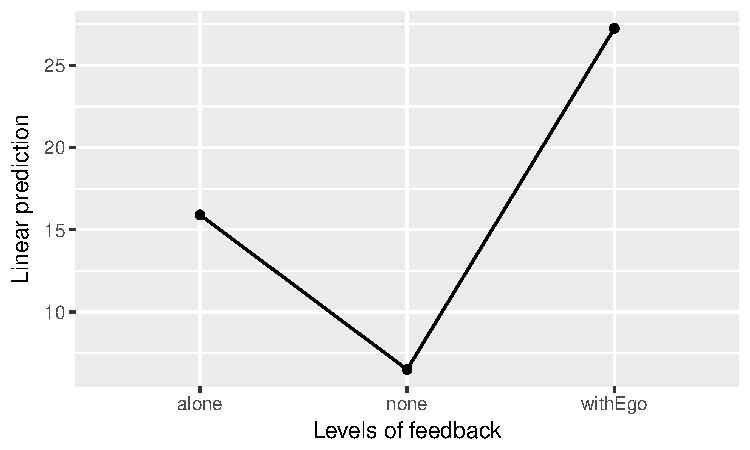
\includegraphics{Unit_5_assignment_KEY_R__spr18__files/figure-latex/unnamed-chunk-65-1} \end{center}

\clearpage

\begin{Shaded}
\begin{Highlighting}[]
\CommentTok{# Mixed ANOVA: post hoc pairwise tests <-- difficulty}
\NormalTok{fit_ano }\OperatorTok\StringTok{ }
\StringTok{  }\NormalTok{emmeans}\OperatorTok{::}\KeywordTok{emmeans}\NormalTok{(}\OperatorTok{~}\StringTok{ }\NormalTok{difficulty) }\OperatorTok\StringTok{ }
\StringTok{  }\KeywordTok{pairs}\NormalTok{(}\DataTypeTok{adjust =} \StringTok{"tukey"}\NormalTok{)}
\end{Highlighting}
\end{Shaded}

\begin{verbatim}
 contrast estimate        SE df t.ratio p.value
 X5 - X6  2.888889 0.4327156 18   6.676  <.0001
 X5 - X7  5.666667 0.4327156 18  13.096  <.0001
 X5 - X8  7.888889 0.4327156 18  18.231  <.0001
 X6 - X7  2.777778 0.4327156 18   6.419  <.0001
 X6 - X8  5.000000 0.4327156 18  11.555  <.0001
 X7 - X8  2.222222 0.4327156 18   5.136  0.0004

Results are averaged over the levels of: feedback 
P value adjustment: tukey method for comparing a family of 4 estimates 
\end{verbatim}

\begin{center}\rule{0.5\linewidth}{\linethickness}\end{center}

\begin{Shaded}
\begin{Highlighting}[]
\CommentTok{# RM ANOVA: means plot <-- difficulty}
\NormalTok{fit_ano }\OperatorTok\StringTok{ }
\StringTok{  }\NormalTok{emmeans}\OperatorTok{::}\KeywordTok{emmip}\NormalTok{( }\OperatorTok{~}\StringTok{ }\NormalTok{difficulty)}
\end{Highlighting}
\end{Shaded}

\begin{center}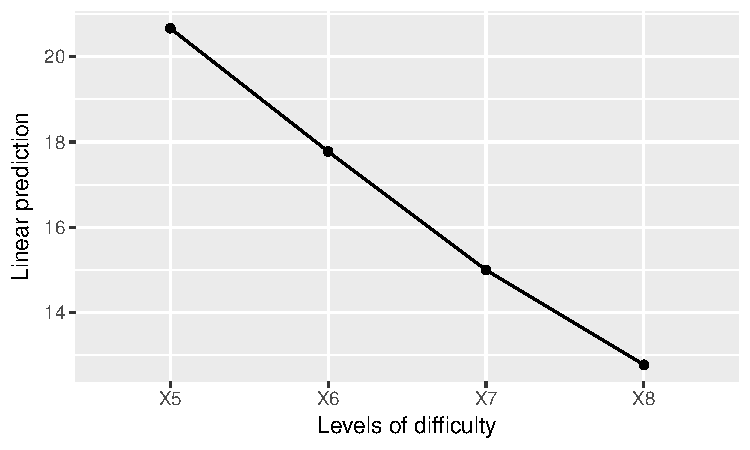
\includegraphics{Unit_5_assignment_KEY_R__spr18__files/figure-latex/unnamed-chunk-67-1} \end{center}

\clearpage

\subsection{\texorpdfstring{\texttt{brain\_wide} - Repeated Measures and
Observed Groups Design: Differential Effect of Stimuli on Recall, by
Brain
Damage}{brain\_wide - Repeated Measures and Observed Groups Design: Differential Effect of Stimuli on Recall, by Brain Damage}}\label{brain_wide---repeated-measures-and-observed-groups-design-differential-effect-of-stimuli-on-recall-by-brain-damage}

\textbf{TEXTBOOK QUESTION:} \emph{Exercise 15B6 described a
neuropsychologist studying subjects with brain damage to the left
cerebral hemisphere. Such a study would probably include a group of
subjects with damage to the right hemisphere and a group of control
subjects without brain damage. The data from Exercise 15B6 (the number
of digit or letter strings each subject recalled) follow, along with
data for the two comparison groups just mentioned.}

\begin{Shaded}
\begin{Highlighting}[]
\NormalTok{brain_wide}
\end{Highlighting}
\end{Shaded}

\begin{verbatim}
  left_digit left_letter left_mixed right_digit right_letter right_mixed
1          6           5          6           9            8           6
2          8           7          5           8            8           7
3          7           7          4           9            7           8
4          8           5          8           7            8           8
5          6           4          7           7            6           7
6          7           6          5           9            8           9
  none_digit none_letter none_mixed
1          8           8          7
2         10           9          9
3          9          10          8
4          9           7          9
5          8           8          8
6         10          10          9
\end{verbatim}

\begin{center}\rule{0.5\linewidth}{\linethickness}\end{center}

Restructure from wide to long format:

\begin{verbatim}
   id damage stimuli longest_correct
1   1   left   digit               6
2   2   left   digit               8
3   3   left   digit               7
4   4   left   digit               8
5   5   left   digit               6
6   6   left   digit               7
7   1   left  letter               5
8   2   left  letter               7
9   3   left  letter               7
10  4   left  letter               5
11  5   left  letter               4
12  6   left  letter               6
13  1   left   mixed               6
14  2   left   mixed               5
15  3   left   mixed               4
16  4   left   mixed               8
17  5   left   mixed               7
18  6   left   mixed               5
19  7  right   digit               9
20  8  right   digit               8
\end{verbatim}

\clearpage

\textbf{Summary Statistics}

\begin{longtable}[]{@{}cccc@{}}
\toprule
\begin{minipage}[b]{0.11\columnwidth}\centering\strut
damage\strut
\end{minipage} & \begin{minipage}[b]{0.17\columnwidth}\centering\strut
digit\strut
\end{minipage} & \begin{minipage}[b]{0.17\columnwidth}\centering\strut
letter\strut
\end{minipage} & \begin{minipage}[b]{0.17\columnwidth}\centering\strut
mixed\strut
\end{minipage}\tabularnewline
\midrule
\endhead
\begin{minipage}[t]{0.11\columnwidth}\centering\strut
left\strut
\end{minipage} & \begin{minipage}[t]{0.17\columnwidth}\centering\strut
7 (0.89)\strut
\end{minipage} & \begin{minipage}[t]{0.17\columnwidth}\centering\strut
5.67 (1.21)\strut
\end{minipage} & \begin{minipage}[t]{0.17\columnwidth}\centering\strut
5.83 (1.47)\strut
\end{minipage}\tabularnewline
\begin{minipage}[t]{0.11\columnwidth}\centering\strut
none\strut
\end{minipage} & \begin{minipage}[t]{0.17\columnwidth}\centering\strut
9 (0.89)\strut
\end{minipage} & \begin{minipage}[t]{0.17\columnwidth}\centering\strut
8.67 (1.21)\strut
\end{minipage} & \begin{minipage}[t]{0.17\columnwidth}\centering\strut
8.33 (0.82)\strut
\end{minipage}\tabularnewline
\begin{minipage}[t]{0.11\columnwidth}\centering\strut
right\strut
\end{minipage} & \begin{minipage}[t]{0.17\columnwidth}\centering\strut
8.17 (0.98)\strut
\end{minipage} & \begin{minipage}[t]{0.17\columnwidth}\centering\strut
7.5 (0.84)\strut
\end{minipage} & \begin{minipage}[t]{0.17\columnwidth}\centering\strut
7.5 (1.05)\strut
\end{minipage}\tabularnewline
\bottomrule
\end{longtable}

\textbf{Profile Plots (raw data)}

\begin{center}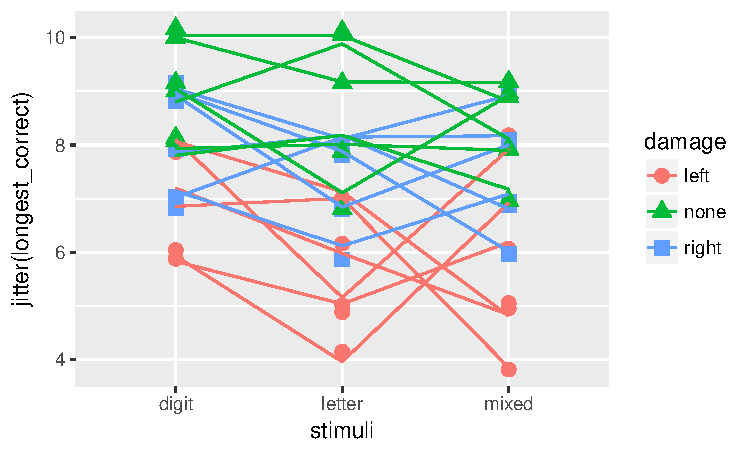
\includegraphics{Unit_5_assignment_KEY_R__spr18__files/figure-latex/unnamed-chunk-71-1} \end{center}

\textbf{Means Plots (raw data)}

\begin{center}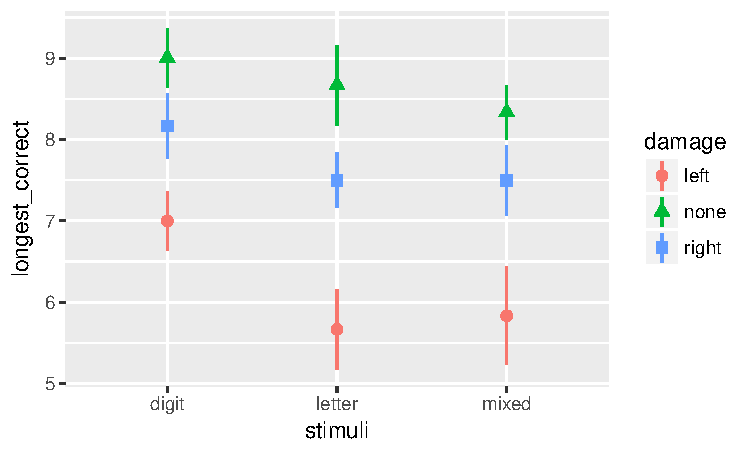
\includegraphics{Unit_5_assignment_KEY_R__spr18__files/figure-latex/unnamed-chunk-72-1} \end{center}

\clearpage

\subsubsection{16B-8a-b Mixed Design ANOVA: with sphericity test and
corrections}\label{b-8a-b-mixed-design-anova-with-sphericity-test-and-corrections}

\textbf{TEXTBOOK QUESTION:} \emph{(a) Perform a mixed-design ANOVA and
test the three F ratios at the .05 level. What can you conclude about
the effects of brain damage on short-term recall for these types of
stimuli? (b) Draw a graph of these data, subject by subject. Do the
assumptions of the mixed-design ANOVA seem reasonable in this case?
Explain. }

\textbf{DIRECTIONS:} Perform a Repeated Measures ANOVA for longest
correct recall under the various stimuli to see if there is an effect
and if the effect is different dependtion on brain damage. Make sure to
save your model (\texttt{fit\_brain}), so that you can use the
\texttt{summary()} function on the name to test for sphericity and make
appropriate corrections.

\begin{Shaded}
\begin{Highlighting}[]
\CommentTok{# Mixe ANOVA:  with sphericity tests and corrections}
\NormalTok{fit_brain <-}\StringTok{ }\NormalTok{brain_long }\OperatorTok\StringTok{   }
\StringTok{  }\NormalTok{afex}\OperatorTok{::}\KeywordTok{aov_4}\NormalTok{(longest_correct }\OperatorTok{~}\StringTok{ }\NormalTok{damage }\OperatorTok{+}\StringTok{ }\NormalTok{(stimuli}\OperatorTok{|}\NormalTok{id),}
            \DataTypeTok{data =}\NormalTok{ .) }

\KeywordTok{summary}\NormalTok{(fit_brain)}
\end{Highlighting}
\end{Shaded}

\begin{verbatim}

Univariate Type III Repeated-Measures ANOVA Assuming Sphericity

                    SS num Df Error SS den Df         F    Pr(>F)    
(Intercept)    3052.52      1   20.111     15 2276.7403 < 2.2e-16 ***
damage           57.37      2   20.111     15   21.3950 4.044e-05 ***
stimuli           7.81      2   30.556     30    3.8364   0.03284 *  
damage:stimuli    1.63      4   30.556     30    0.4000   0.80705    
---
Signif. codes:  0 '***' 0.001 '**' 0.01 '*' 0.05 '.' 0.1 ' ' 1


Mauchly Tests for Sphericity

               Test statistic  p-value
stimuli               0.55585 0.016394
damage:stimuli        0.55585 0.016394


Greenhouse-Geisser and Huynh-Feldt Corrections
 for Departure from Sphericity

                GG eps Pr(>F[GG])  
stimuli        0.69245    0.05194 .
damage:stimuli 0.69245    0.73932  
---
Signif. codes:  0 '***' 0.001 '**' 0.01 '*' 0.05 '.' 0.1 ' ' 1

                  HF eps Pr(>F[HF])
stimuli        0.7402929 0.04836111
damage:stimuli 0.7402929 0.75188515
\end{verbatim}

\clearpage

\subsubsection{16B-8c Mixed Design ANOVA: Main Effect's post-hoc with
appropriate
correction}\label{b-8c-mixed-design-anova-main-effects-post-hoc-with-appropriate-correction}

\textbf{TEXTBOOK QUESTION:} \emph{(c) Perform post hoc pairwise
comparisons for both main effects. Do not assume sphericity for the RM
factor.}

\textbf{DIRECTIONS:} Use the prior model \texttt{fit\_brain} to run post
hoc test for the levels of each main effect, separately SINCE THE
INTERACTION IS NOT SIGNIFICANT (including a means plot). Choose an
appropriate method to control type I errors when making multiple
comparisons. (you do not need to worry about sphericity)

\begin{Shaded}
\begin{Highlighting}[]
\CommentTok{# Mixed ANOVA: post hoc pairwise tests <-- damage}
\NormalTok{fit_brain }\OperatorTok\StringTok{ }
\StringTok{  }\NormalTok{emmeans}\OperatorTok{::}\KeywordTok{emmeans}\NormalTok{(}\OperatorTok{~}\StringTok{ }\NormalTok{damage) }\OperatorTok\StringTok{ }
\StringTok{  }\KeywordTok{pairs}\NormalTok{(}\DataTypeTok{adjust =} \StringTok{"none"}\NormalTok{)}
\end{Highlighting}
\end{Shaded}

\begin{verbatim}
 contrast       estimate        SE df t.ratio p.value
 left - none  -2.5000000 0.3859679 15  -6.477  <.0001
 left - right -1.5555556 0.3859679 15  -4.030  0.0011
 none - right  0.9444444 0.3859679 15   2.447  0.0272

Results are averaged over the levels of: stimuli 
\end{verbatim}

\begin{center}\rule{0.5\linewidth}{\linethickness}\end{center}

\begin{Shaded}
\begin{Highlighting}[]
\CommentTok{# RM ANOVA: means plot <-- damage}
\NormalTok{fit_brain }\OperatorTok
\StringTok{  }\NormalTok{emmeans}\OperatorTok{::}\KeywordTok{emmip}\NormalTok{( }\OperatorTok{~}\StringTok{ }\NormalTok{damage)}
\end{Highlighting}
\end{Shaded}

\begin{center}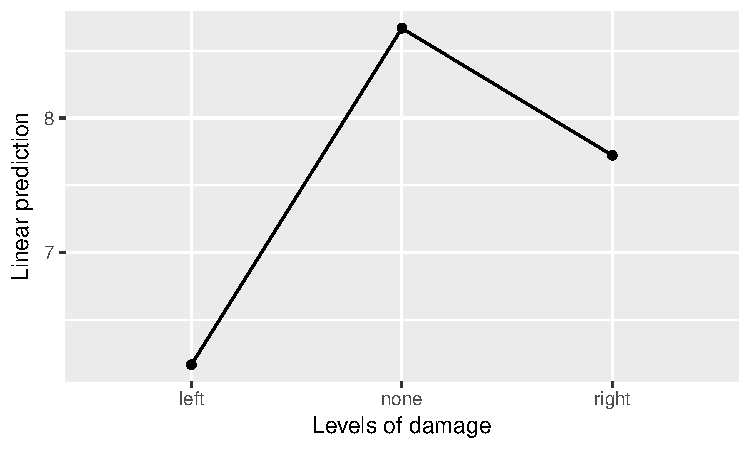
\includegraphics{Unit_5_assignment_KEY_R__spr18__files/figure-latex/unnamed-chunk-75-1} \end{center}

\clearpage

\begin{Shaded}
\begin{Highlighting}[]
\CommentTok{# Mixed ANOVA: post hoc pairwise tests <-- stimuli}
\NormalTok{fit_brain }\OperatorTok\StringTok{ }
\StringTok{  }\NormalTok{emmeans}\OperatorTok{::}\KeywordTok{emmeans}\NormalTok{(}\OperatorTok{~}\StringTok{ }\NormalTok{stimuli) }\OperatorTok\StringTok{ }
\StringTok{  }\KeywordTok{pairs}\NormalTok{(}\DataTypeTok{adjust =} \StringTok{"none"}\NormalTok{)}
\end{Highlighting}
\end{Shaded}

\begin{verbatim}
 contrast         estimate        SE df t.ratio p.value
 digit - letter 0.77777778 0.3364056 30   2.312  0.0278
 digit - mixed  0.83333333 0.3364056 30   2.477  0.0191
 letter - mixed 0.05555556 0.3364056 30   0.165  0.8699

Results are averaged over the levels of: damage 
\end{verbatim}

\begin{center}\rule{0.5\linewidth}{\linethickness}\end{center}

\begin{Shaded}
\begin{Highlighting}[]
\CommentTok{# RM ANOVA: means plot <-- stimuli}
\NormalTok{fit_brain }\OperatorTok
\StringTok{  }\NormalTok{emmeans}\OperatorTok{::}\KeywordTok{emmip}\NormalTok{( }\OperatorTok{~}\StringTok{ }\NormalTok{stimuli)}
\end{Highlighting}
\end{Shaded}

\begin{center}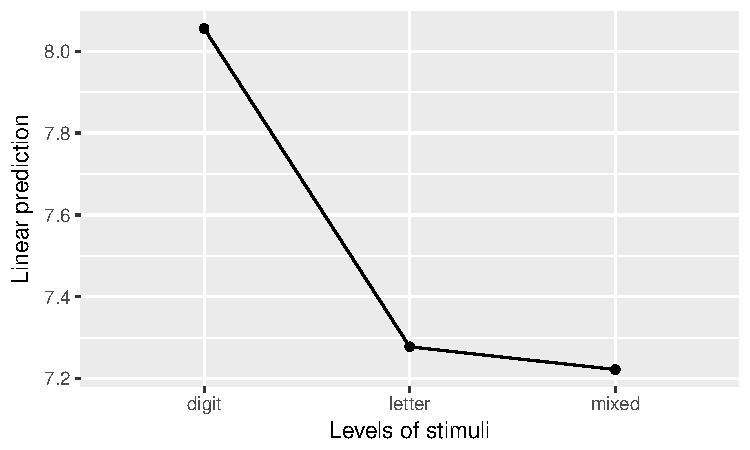
\includegraphics{Unit_5_assignment_KEY_R__spr18__files/figure-latex/unnamed-chunk-77-1} \end{center}

\clearpage

\subsection{\texorpdfstring{\texttt{ihno\_clean} - Repeated Measures and
Observed Group Design: Differential Effect of Time on Anxiety, by
Major}{ihno\_clean - Repeated Measures and Observed Group Design: Differential Effect of Time on Anxiety, by Major}}\label{ihno_clean---repeated-measures-and-observed-group-design-differential-effect-of-time-on-anxiety-by-major}

\subsubsection{16c-1a Mixed Design ANOVA: with main effect post
hocs}\label{c-1a-mixed-design-anova-with-main-effect-post-hocs}

\textbf{TEXTBOOK QUESTION:} \emph{(a) Perform a mixed-design ANOVA with
the three anxiety measures as the RM levels, and major as the
between-subjects factor. Request a plot of the cell means, \sout{and
post hoc tests for both the RM factor (LSD) and for major (Tukey)}.
Report the results of the ANOVA in APA style.}

\textbf{DIRECTIONS:} Using the \texttt{ihno\_anx\_long} dataset from the
chapter 15 questions, perform a Repeated Measures ANOVA for at the three
time points to see if the experiment had an effect on anxiety and if the
effect is different dependtion on major. Make sure to save your model
(\texttt{fit\_anx\_major}), so that you can use the \texttt{summary()}
function on the name to test for sphericity and make appropriate
corrections. Do specify that you would like to display BOTH effect size
measures with \texttt{es\ =\ c("ges",\ "pes")}, but do NOT include
\texttt{correction\ =\ "none"}.

\begin{Shaded}
\begin{Highlighting}[]
\CommentTok{# Mixe ANOVA:  with sphericity tests and corrections}
\NormalTok{fit_anx_major <-}\StringTok{ }\NormalTok{ihno_anx_long }\OperatorTok\StringTok{   }
\StringTok{  }\NormalTok{afex}\OperatorTok{::}\KeywordTok{aov_4}\NormalTok{(anxiety }\OperatorTok{~}\StringTok{ }\NormalTok{majorF }\OperatorTok{+}\StringTok{ }\NormalTok{(time}\OperatorTok{|}\NormalTok{sub_num),}
            \DataTypeTok{data =}\NormalTok{ .,}
            \DataTypeTok{anova_table =} \KeywordTok{list}\NormalTok{(}\DataTypeTok{es =} \KeywordTok{c}\NormalTok{(}\StringTok{"ges"}\NormalTok{, }\StringTok{"pes"}\NormalTok{)))}

\KeywordTok{summary}\NormalTok{(fit_anx_major)}
\end{Highlighting}
\end{Shaded}

\begin{verbatim}

Univariate Type III Repeated-Measures ANOVA Assuming Sphericity

               SS num Df Error SS den Df         F  Pr(>F)    
(Intercept) 94251      1   5528.2     95 1619.6712 < 2e-16 ***
majorF        653      4   5528.2     95    2.8063 0.02990 *  
time           44      2   1851.2    190    2.2486 0.10835    
majorF:time   172      8   1851.2    190    2.2098 0.02841 *  
---
Signif. codes:  0 '***' 0.001 '**' 0.01 '*' 0.05 '.' 0.1 ' ' 1


Mauchly Tests for Sphericity

            Test statistic    p-value
time               0.81322 6.0211e-05
majorF:time        0.81322 6.0211e-05


Greenhouse-Geisser and Huynh-Feldt Corrections
 for Departure from Sphericity

             GG eps Pr(>F[GG])  
time        0.84261    0.11753  
majorF:time 0.84261    0.03812 *
---
Signif. codes:  0 '***' 0.001 '**' 0.01 '*' 0.05 '.' 0.1 ' ' 1

               HF eps Pr(>F[HF])
time        0.8561438 0.11672523
majorF:time 0.8561438 0.03715744
\end{verbatim}

\clearpage

\textbf{DIRECTIONS:} To display the effect size meausre, run the name
(\texttt{fit\_anx\_major}) of the model alone.

\begin{Shaded}
\begin{Highlighting}[]
\NormalTok{fit_anx_major}
\end{Highlighting}
\end{Shaded}

\begin{verbatim}
Anova Table (Type 3 tests)

Response: anxiety
       Effect           df   MSE      F  ges pes p.value
1      majorF        4, 95 58.19 2.81 *  .08 .11     .03
2        time 1.69, 160.10 11.56   2.25 .006 .02     .12
3 majorF:time 6.74, 160.10 11.56 2.21 *  .02 .09     .04
---
Signif. codes:  0 '***' 0.001 '**' 0.01 '*' 0.05 '+' 0.1 ' ' 1

Sphericity correction method: GG 
\end{verbatim}

\begin{center}\rule{0.5\linewidth}{\linethickness}\end{center}

\textbf{DIRECTIONS:} SINCE THE INTERACTIONIS SIGNIFICANT, instead of
focusing on the main effects alone, plot the interaction with the
\texttt{emmeans::emmip(group\_var\ \textasciitilde{}\ RM\_var)}
function.

\begin{Shaded}
\begin{Highlighting}[]
\CommentTok{# RM ANOVA: means plot <-- interaction}
\NormalTok{fit_anx_major }\OperatorTok
\StringTok{  }\NormalTok{emmeans}\OperatorTok{::}\KeywordTok{emmip}\NormalTok{(majorF }\OperatorTok{~}\StringTok{ }\NormalTok{time)}
\end{Highlighting}
\end{Shaded}

\begin{center}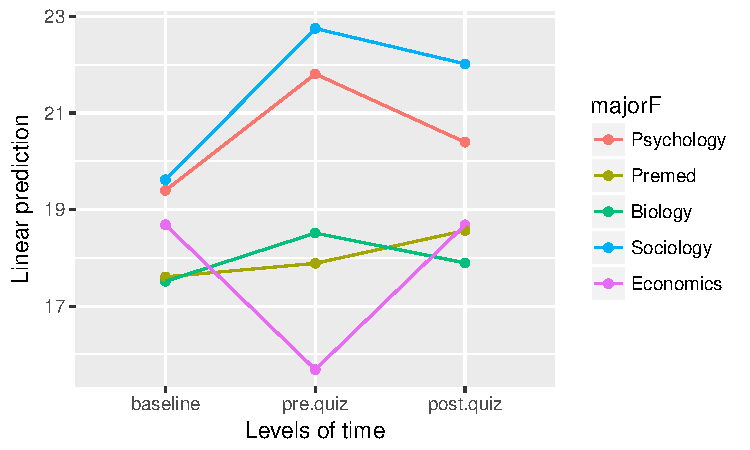
\includegraphics{Unit_5_assignment_KEY_R__spr18__files/figure-latex/unnamed-chunk-80-1} \end{center}

\clearpage

\subsection{\texorpdfstring{\texttt{ihno\_clean} - Repeated Measures and
Observed Group Design: Differential Effect of a Pop Quiz (Time =
Baseline, pre-quiz, post-quiz) on Heart Rate, by
Gender}{ihno\_clean - Repeated Measures and Observed Group Design: Differential Effect of a Pop Quiz (Time = Baseline, pre-quiz, post-quiz) on Heart Rate, by Gender}}\label{ihno_clean---repeated-measures-and-observed-group-design-differential-effect-of-a-pop-quiz-time-baseline-pre-quiz-post-quiz-on-heart-rate-by-gender}

\subsubsection{16c-2a Mixed Design ANOVA: with main effect post
hocs}\label{c-2a-mixed-design-anova-with-main-effect-post-hocs}

\textbf{TEXTBOOK QUESTION:} \emph{(a) Perform a mixed-design ANOVA with
the three heart-rate measures as the RM levels and gender as the
between-subjects factor. Request a plot of the cell means and post hoc
tests for the RM factor (LSD). Report the results of the ANOVA in APA
style.}

\begin{Shaded}
\begin{Highlighting}[]
\NormalTok{ihno_clean }\OperatorTok\StringTok{ }
\StringTok{  }\NormalTok{dplyr}\OperatorTok{::}\KeywordTok{select}\NormalTok{(sub_num, genderF, hr_base, hr_pre, hr_post) }\OperatorTok\StringTok{ }
\StringTok{  }\KeywordTok{head}\NormalTok{(}\DataTypeTok{n =} \DecValTok{4}\NormalTok{)}
\end{Highlighting}
\end{Shaded}

\begin{verbatim}
# A tibble: 4 x 5
  sub_num genderF hr_base hr_pre hr_post
    <dbl> <fct>     <dbl>  <dbl>   <dbl>
1    1.00 Female     71.0   68.0    65.0
2    2.00 Female     73.0   75.0    68.0
3    3.00 Female     69.0   76.0    72.0
4    4.00 Female     72.0   73.0    78.0
\end{verbatim}

Restructure from wide to long format:

\begin{Shaded}
\begin{Highlighting}[]
\CommentTok{#Restructure: wide-to-long}
\NormalTok{ihno_hr_long <-}\StringTok{ }\NormalTok{ihno_clean }\OperatorTok\StringTok{ }
\StringTok{  }\NormalTok{tidyr}\OperatorTok{::}\KeywordTok{gather}\NormalTok{(}\DataTypeTok{key =}\NormalTok{ variable,}
                \DataTypeTok{value =}\NormalTok{ hr,}
\NormalTok{                hr_base, hr_pre, hr_post) }\OperatorTok\StringTok{ }
\StringTok{  }\NormalTok{dplyr}\OperatorTok{::}\KeywordTok{mutate}\NormalTok{(}\DataTypeTok{time =} \KeywordTok{case_when}\NormalTok{(variable }\OperatorTok{==}\StringTok{ "hr_base"} \OperatorTok{~}\StringTok{ "baseline"}\NormalTok{,}
\NormalTok{                                 variable }\OperatorTok{==}\StringTok{ "hr_pre"}  \OperatorTok{~}\StringTok{ "pre-quiz"}\NormalTok{,}
\NormalTok{                                 variable }\OperatorTok{==}\StringTok{ "hr_post"} \OperatorTok{~}\StringTok{ "post-quiz"}\NormalTok{) }\OperatorTok\StringTok{ }
\StringTok{                  }\KeywordTok{factor}\NormalTok{(}\DataTypeTok{levels =} \KeywordTok{c}\NormalTok{(}\StringTok{"baseline"}\NormalTok{, }\StringTok{"pre-quiz"}\NormalTok{, }\StringTok{"post-quiz"}\NormalTok{))) }\OperatorTok\StringTok{ }
\StringTok{  }\NormalTok{dplyr}\OperatorTok{::}\KeywordTok{arrange}\NormalTok{(sub_num, time)}
\end{Highlighting}
\end{Shaded}

\begin{Shaded}
\begin{Highlighting}[]
\NormalTok{ihno_hr_long }\OperatorTok\StringTok{ }
\StringTok{  }\NormalTok{dplyr}\OperatorTok{::}\KeywordTok{select}\NormalTok{(sub_num, genderF, time, hr) }\OperatorTok\StringTok{ }
\StringTok{  }\KeywordTok{head}\NormalTok{(}\DataTypeTok{n =} \DecValTok{12}\NormalTok{)}
\end{Highlighting}
\end{Shaded}

\begin{verbatim}
# A tibble: 12 x 4
   sub_num genderF time         hr
     <dbl> <fct>   <fct>     <dbl>
 1    1.00 Female  baseline   71.0
 2    1.00 Female  pre-quiz   68.0
 3    1.00 Female  post-quiz  65.0
 4    2.00 Female  baseline   73.0
 5    2.00 Female  pre-quiz   75.0
 6    2.00 Female  post-quiz  68.0
 7    3.00 Female  baseline   69.0
 8    3.00 Female  pre-quiz   76.0
 9    3.00 Female  post-quiz  72.0
10    4.00 Female  baseline   72.0
11    4.00 Female  pre-quiz   73.0
12    4.00 Female  post-quiz  78.0
\end{verbatim}

\clearpage

\textbf{DIRECTIONS:} Using the \texttt{ihno\_hr\_long} dataset just
reformatted, perform a Repeated Measures ANOVA for at the three time
points to see if the experiment had an effect on heart rateand if the
effect is different dependtion on gender Make sure to save your model
(\texttt{fit\_hr\_major}), so that you can use the \texttt{summary()}
function on the name to test for sphericity and make appropriate
corrections. Do specify that you would like to display BOTH effect size
measures with \texttt{es\ =\ c("ges",\ "pes")}, but do NOT include
\texttt{correction\ =\ "none"}.

\begin{Shaded}
\begin{Highlighting}[]
\CommentTok{# Mixe ANOVA:  with sphericity tests and corrections}
\NormalTok{fit_hr_major <-}\StringTok{ }\NormalTok{ihno_hr_long }\OperatorTok\StringTok{   }
\StringTok{  }\NormalTok{afex}\OperatorTok{::}\KeywordTok{aov_4}\NormalTok{(hr }\OperatorTok{~}\StringTok{ }\NormalTok{genderF }\OperatorTok{+}\StringTok{ }\NormalTok{(time}\OperatorTok{|}\NormalTok{sub_num),}
            \DataTypeTok{data =}\NormalTok{ .,}
            \DataTypeTok{anova_table =} \KeywordTok{list}\NormalTok{(}\DataTypeTok{es =} \KeywordTok{c}\NormalTok{(}\StringTok{"ges"}\NormalTok{, }\StringTok{"pes"}\NormalTok{)))}

\KeywordTok{summary}\NormalTok{(fit_hr_major)}
\end{Highlighting}
\end{Shaded}

\begin{verbatim}

Univariate Type III Repeated-Measures ANOVA Assuming Sphericity

                  SS num Df Error SS den Df          F    Pr(>F)    
(Intercept)  1560400      1   3460.1     98 44195.5684 < 2.2e-16 ***
genderF          276      1   3460.1     98     7.8284  0.006193 ** 
time             130      2   2109.7    196     6.0357  0.002859 ** 
genderF:time       8      2   2109.7    196     0.3871  0.679572    
---
Signif. codes:  0 '***' 0.001 '**' 0.01 '*' 0.05 '.' 0.1 ' ' 1


Mauchly Tests for Sphericity

             Test statistic p-value
time                0.99258 0.69671
genderF:time        0.99258 0.69671


Greenhouse-Geisser and Huynh-Feldt Corrections
 for Departure from Sphericity

              GG eps Pr(>F[GG])   
time         0.99263   0.002932 **
genderF:time 0.99263   0.678033   
---
Signif. codes:  0 '***' 0.001 '**' 0.01 '*' 0.05 '.' 0.1 ' ' 1

               HF eps  Pr(>F[HF])
time         1.013079 0.002859441
genderF:time 1.013079 0.679571523
\end{verbatim}

\clearpage

\textbf{DIRECTIONS:} Use the prior model \texttt{fit\_brain} to run post
hoc test for the levels of each main effect, separately SINCE THE
INTERACTION IS NOT SIGNIFICANT (including a means plot). Choose an
appropriate method to control type I errors when making multiple
comparisons. (you do not need to worry about sphericity)

\begin{Shaded}
\begin{Highlighting}[]
\CommentTok{# Mixed ANOVA: post hoc pairwise tests <-- damage}
\NormalTok{fit_hr_major }\OperatorTok\StringTok{ }
\StringTok{  }\NormalTok{emmeans}\OperatorTok{::}\KeywordTok{emmeans}\NormalTok{(}\OperatorTok{~}\StringTok{ }\NormalTok{time) }\OperatorTok\StringTok{ }
\StringTok{  }\KeywordTok{pairs}\NormalTok{(}\DataTypeTok{adjust =} \StringTok{"none"}\NormalTok{)}
\end{Highlighting}
\end{Shaded}

\begin{verbatim}
 contrast               estimate      SE  df t.ratio p.value
 baseline - pre.quiz  -1.6087311 0.46859 196  -3.433  0.0007
 baseline - post.quiz -0.5877193 0.46859 196  -1.254  0.2113
 pre.quiz - post.quiz  1.0210118 0.46859 196   2.179  0.0305

Results are averaged over the levels of: genderF 
\end{verbatim}

\begin{center}\rule{0.5\linewidth}{\linethickness}\end{center}

\begin{Shaded}
\begin{Highlighting}[]
\CommentTok{# RM ANOVA: means plot <-- damage}
\NormalTok{fit_hr_major }\OperatorTok
\StringTok{  }\NormalTok{emmeans}\OperatorTok{::}\KeywordTok{emmip}\NormalTok{( }\OperatorTok{~}\StringTok{ }\NormalTok{time)}
\end{Highlighting}
\end{Shaded}

\begin{center}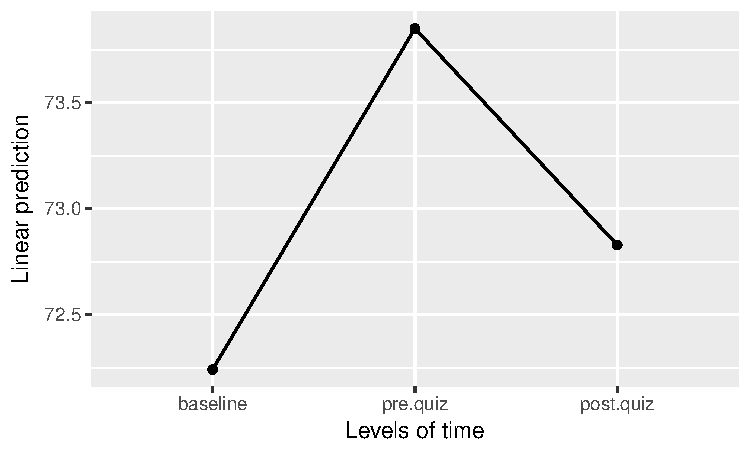
\includegraphics{Unit_5_assignment_KEY_R__spr18__files/figure-latex/unnamed-chunk-86-1} \end{center}

\clearpage

\begin{Shaded}
\begin{Highlighting}[]
\CommentTok{# Mixed ANOVA: post hoc pairwise tests <-- genderF}
\NormalTok{fit_hr_major }\OperatorTok\StringTok{ }
\StringTok{  }\NormalTok{emmeans}\OperatorTok{::}\KeywordTok{emmeans}\NormalTok{(}\OperatorTok{~}\StringTok{ }\NormalTok{genderF) }\OperatorTok\StringTok{ }
\StringTok{  }\KeywordTok{pairs}\NormalTok{(}\DataTypeTok{adjust =} \StringTok{"none"}\NormalTok{)}
\end{Highlighting}
\end{Shaded}

\begin{verbatim}
 contrast      estimate        SE df t.ratio p.value
 Female - Male   1.9388 0.6929412 98   2.798  0.0062

Results are averaged over the levels of: time 
\end{verbatim}

\begin{center}\rule{0.5\linewidth}{\linethickness}\end{center}

\begin{Shaded}
\begin{Highlighting}[]
\CommentTok{# RM ANOVA: means plot <-- stimuli}
\NormalTok{fit_hr_major }\OperatorTok
\StringTok{  }\NormalTok{emmeans}\OperatorTok{::}\KeywordTok{emmip}\NormalTok{( }\OperatorTok{~}\StringTok{ }\NormalTok{genderF)}
\end{Highlighting}
\end{Shaded}

\begin{center}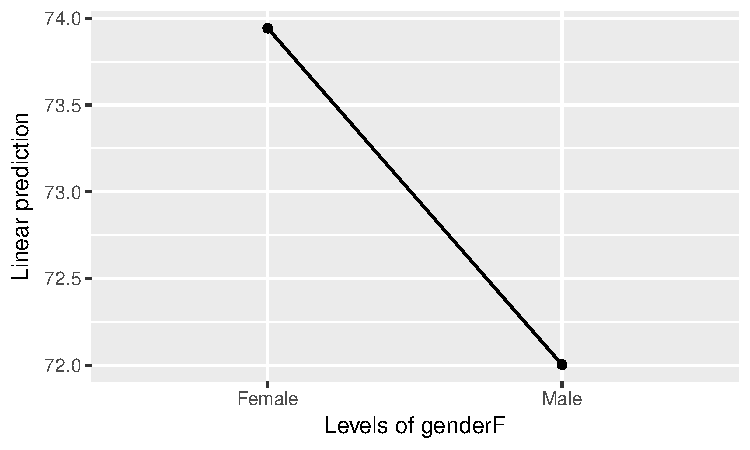
\includegraphics{Unit_5_assignment_KEY_R__spr18__files/figure-latex/unnamed-chunk-88-1} \end{center}

\clearpage

\subsection{\texorpdfstring{\texttt{ihno\_clean} - Repeated Measures and
Assigned Group Design: Differential Effect of the Experiemnt (Time = Pop
Quiz vs.~Standard Quiz) on Quiz Score, by Difficulty
Level}{ihno\_clean - Repeated Measures and Assigned Group Design: Differential Effect of the Experiemnt (Time = Pop Quiz vs.~Standard Quiz) on Quiz Score, by Difficulty Level}}\label{ihno_clean---repeated-measures-and-assigned-group-design-differential-effect-of-the-experiemnt-time-pop-quiz-vs.standard-quiz-on-quiz-score-by-difficulty-level}

\subsubsection{16c-3a Mixed Design ANOVA: is there an
interaction?}\label{c-3a-mixed-design-anova-is-there-an-interaction}

\textbf{TEXTBOOK QUESTION:} \emph{(a) Perform a mixed-design ANOVA with
the two 10-point quizzes (statquiz and exp\_sqz) as the RM levels, and
exp\_cond as the between-subjects factor. Request a plot of the cell
means. Report the results of the ANOVA in APA style. If the interaction
is significant, explain the pattern you see in the plot of the cell
means.}

\textbf{DIRECTIONS:} Using the \texttt{ihno\_statquiz\_long} dataset
from the chapter 15 questions, perform a Repeated Measures ANOVA for at
the two quizes to see if the experiment had an effect on score and if
the effect is different dependtion on difficulty level. Make sure to
save your model (\texttt{fit\_anx\_major}), so that you can use the
\texttt{summary()} function on the name to view the output. Do specify
that you would like to display BOTH effect size measures with
\texttt{es\ =\ c("ges",\ "pes")}, but do NOT include
\texttt{correction\ =\ "none"}.

\begin{quote}
NOTE: When the measure is only repeated twice, sphericity can not be
violated, so no such test are performed.
\end{quote}

\begin{Shaded}
\begin{Highlighting}[]
\CommentTok{# Mixed ANOVA:  with summary}
\NormalTok{fit_statquiz <-}\StringTok{ }\NormalTok{ihno_statquiz_long }\OperatorTok\StringTok{   }
\StringTok{  }\NormalTok{afex}\OperatorTok{::}\KeywordTok{aov_4}\NormalTok{(s_quiz }\OperatorTok{~}\StringTok{ }\NormalTok{exp_condF }\OperatorTok{+}\StringTok{ }\NormalTok{(time}\OperatorTok{|}\NormalTok{sub_num),}
            \DataTypeTok{data =}\NormalTok{ .,}
            \DataTypeTok{anova_table =} \KeywordTok{list}\NormalTok{(}\DataTypeTok{es =} \KeywordTok{c}\NormalTok{(}\StringTok{"ges"}\NormalTok{, }\StringTok{"pes"}\NormalTok{)))}

\KeywordTok{summary}\NormalTok{(fit_statquiz)}
\end{Highlighting}
\end{Shaded}

\begin{verbatim}

Univariate Type III Repeated-Measures ANOVA Assuming Sphericity

                   SS num Df Error SS den Df         F    Pr(>F)    
(Intercept)    9370.8      1   585.28     96 1537.0375 < 2.2e-16 ***
exp_condF        33.4      3   585.28     96    1.8270    0.1474    
time              0.0      1    54.64     96    0.0791    0.7792    
exp_condF:time   54.8      3    54.64     96   32.1025 1.853e-14 ***
---
Signif. codes:  0 '***' 0.001 '**' 0.01 '*' 0.05 '.' 0.1 ' ' 1
\end{verbatim}

\clearpage

\textbf{DIRECTIONS:} SINCE THE INTERACTIONIS SIGNIFICANT, instead of
focusing on the main effects alone, plot the interaction with the
\texttt{emmeans::emmip(group\_var\ \textasciitilde{}\ RM\_var)}
function.

\begin{Shaded}
\begin{Highlighting}[]
\CommentTok{# RM ANOVA: means plot <-- interaction}
\NormalTok{fit_statquiz }\OperatorTok
\StringTok{  }\NormalTok{emmeans}\OperatorTok{::}\KeywordTok{emmip}\NormalTok{(exp_condF }\OperatorTok{~}\StringTok{ }\NormalTok{time)}
\end{Highlighting}
\end{Shaded}

\begin{center}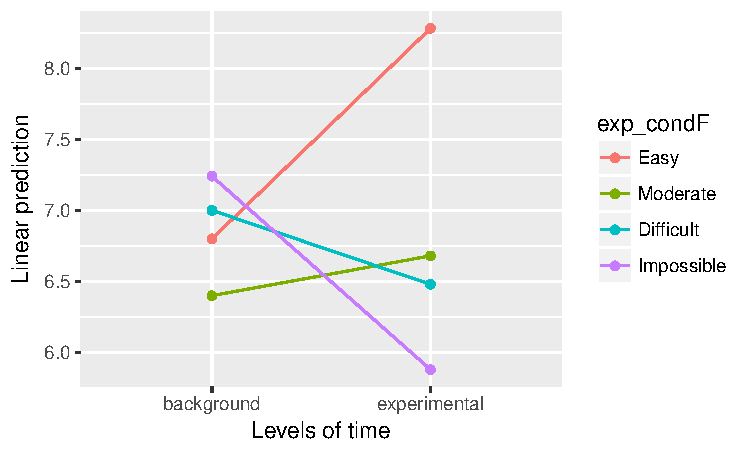
\includegraphics{Unit_5_assignment_KEY_R__spr18__files/figure-latex/unnamed-chunk-90-1} \end{center}


\end{document}
